\PassOptionsToPackage{unicode=true}{hyperref} % options for packages loaded elsewhere
\PassOptionsToPackage{hyphens}{url}
%
\documentclass[]{article}
\usepackage{lmodern}
\usepackage{amssymb,amsmath}
\usepackage{ifxetex,ifluatex}
\usepackage{fixltx2e} % provides \textsubscript
\ifnum 0\ifxetex 1\fi\ifluatex 1\fi=0 % if pdftex
  \usepackage[T1]{fontenc}
  \usepackage[utf8]{inputenc}
  \usepackage{textcomp} % provides euro and other symbols
\else % if luatex or xelatex
  \usepackage{unicode-math}
  \defaultfontfeatures{Ligatures=TeX,Scale=MatchLowercase}
\fi
% use upquote if available, for straight quotes in verbatim environments
\IfFileExists{upquote.sty}{\usepackage{upquote}}{}
% use microtype if available
\IfFileExists{microtype.sty}{%
\usepackage[]{microtype}
\UseMicrotypeSet[protrusion]{basicmath} % disable protrusion for tt fonts
}{}
\IfFileExists{parskip.sty}{%
\usepackage{parskip}
}{% else
\setlength{\parindent}{0pt}
\setlength{\parskip}{6pt plus 2pt minus 1pt}
}
\usepackage{hyperref}
\hypersetup{
            pdftitle={Chainsweep-based efficiency of bottom trawl surveys and biomass estimates for flatfish, red hake, and goosefish stocks in Northwest Atlantic waters of the United States},
            pdfauthor={Timothy J. Miller1, David E. Richardson2, Andrew Jones2, Phil Politis1},
            pdfborder={0 0 0},
            breaklinks=true}
\urlstyle{same}  % don't use monospace font for urls
\usepackage[margin=1in]{geometry}
\usepackage{graphicx,grffile}
\makeatletter
\def\maxwidth{\ifdim\Gin@nat@width>\linewidth\linewidth\else\Gin@nat@width\fi}
\def\maxheight{\ifdim\Gin@nat@height>\textheight\textheight\else\Gin@nat@height\fi}
\makeatother
% Scale images if necessary, so that they will not overflow the page
% margins by default, and it is still possible to overwrite the defaults
% using explicit options in \includegraphics[width, height, ...]{}
\setkeys{Gin}{width=\maxwidth,height=\maxheight,keepaspectratio}
\setlength{\emergencystretch}{3em}  % prevent overfull lines
\providecommand{\tightlist}{%
  \setlength{\itemsep}{0pt}\setlength{\parskip}{0pt}}
\setcounter{secnumdepth}{5}
% Redefines (sub)paragraphs to behave more like sections
\ifx\paragraph\undefined\else
\let\oldparagraph\paragraph
\renewcommand{\paragraph}[1]{\oldparagraph{#1}\mbox{}}
\fi
\ifx\subparagraph\undefined\else
\let\oldsubparagraph\subparagraph
\renewcommand{\subparagraph}[1]{\oldsubparagraph{#1}\mbox{}}
\fi

% set default figure placement to htbp
\makeatletter
\def\fps@figure{htbp}
\makeatother

\usepackage{url}
\usepackage{setspace}
%\singlespacing
%\onehalfspacing
\doublespacing
\usepackage{lineno}
\linenumbers
\usepackage[belowskip=0pt,aboveskip=0pt]{caption}
\usepackage{relsize}
\newcommand{\afrb}{Alaska Fishery Research Bulletin\xspace}
\newcommand{\ajms}{African Journal of Marine Science\xspace}
\newcommand{\amb}{Advances in Marine Biology\xspace}
\newcommand{\bms}{Bulletin of Marine Science\xspace}
\newcommand{\bjssf}{Bulletin of the Japanese Society of Scientific Fisheries\xspace}
\newcommand{\cb}{Conservation Biology\xspace}
\newcommand{\cjfas}{Canadian Journal of Fisheries and Aquatic Sciences\xspace}
\newcommand{\ea}{Ecological Applications\xspace}
\newcommand{\eer}{Evolutionary Ecology Research\xspace}
\newcommand{\elet}{Ecology Letters\xspace}
\newcommand{\emod}{Ecological Modelling\xspace}
\newcommand{\ebf}{Environmental Biology of Fishes\xspace}
\newcommand{\ff}{Fish and Fisheries\xspace}
\newcommand{\fo}{Fisheries Oceanography\xspace}
\newcommand{\fr}{Fisheries Research\xspace}
\newcommand{\fb}{Fishery Bulletin\xspace}
\newcommand{\ijms}{ICES Journal of Marine Science\xspace}
\newcommand{\iccat}{Collective Volume of Scientific Papers ICCAT\xspace}
\newcommand{\jae}{Journal of Animal Ecology\xspace}
\newcommand{\jai}{Journal of Applied Ichthyology\xspace}
\newcommand{\jdc}{Journal Du Conseil International Pour L'exploration De La Mer\xspace}
\newcommand{\jdcp}{Journal Du Conseil Permanent International Pour L'exploration De La Mer\xspace}
\newcommand{\jembe}{Journal of Experimental Marine Biology and Ecology\xspace}
\newcommand{\jfb}{Journal of Fish Biology\xspace}
\newcommand{\jsr}{Journal of Sea Research\xspace}
\newcommand{\jtb}{Journal of Theoretical Biology\xspace}
\newcommand{\jfrbc}{Journal of the Fisheries Research Board of Canada\xspace}
\newcommand{\jnwafs}{Journal of Northwest Atlantic Fisheries Science\xspace}
\newcommand{\mcf}{Marine and Coastal Fisheries: Dynamics, Management, and Ecosystem Science\xspace}
\newcommand{\mb}{Marine Biology\xspace}
\newcommand{\meps}{Marine Ecology Progress Series\xspace}
\newcommand{\mfr}{Marine Fisheries Review\xspace}
\newcommand{\mpb}{Marine Pollution Bulletin\xspace}
\newcommand{\najfm}{North American Journal of Fisheries Management\xspace}
\newcommand{\nzjmfr}{New Zealand Journal of Marine and Freshwater Research\xspace}
\newcommand{\pnas}{Proceedings of the National Academy of Sciences USA\xspace}
\newcommand{\rpvrciemm}{Rapports et Proc\`es-Verbaux des R\'eunions. Conseil Internationale pour l'Exploration de la Mer\xspace}
\newcommand{\rpvrcpiemm}{Rapports et Proc\`es-Verbaux des R\'eunions. Conseil Permanent Internationale pour l'Exploration de la Mer\xspace}
\newcommand{\rfbf}{Reviews in Fish Biology and Fisheries\xspace}
\newcommand{\sajms}{South African Journal of Marine Science\xspace}
\newcommand{\tafs}{Transactions of the American Fisheries Society\xspace}

\newcommand{\anzjs}{Australian \& New Zealand Journal of Statistics\xspace}
\newcommand{\as}{Applied Statistics\xspace}
\newcommand{\csda}{Computational Statistics \& Data Analysis\xspace}
\newcommand{\ees}{Environmental and Ecological Statistics\xspace}
\newcommand{\jas}{Journal of Applied Statistics\xspace}
\newcommand{\jabes}{Journal of Agricultural, Biological, and Environmental Statistics\xspace}
\newcommand{\jasa}{Journal of the American Statistical Association\xspace}
\newcommand{\jrssb}{Journal of the Royal Statistical Society. Series B\xspace}
\newcommand{\sm}{Statistics in Medicine}
\usepackage{xspace}
\usepackage{bm}
\usepackage{caption,graphics}
\usepackage{graphicx}
\usepackage{makecell}
\renewcommand\figurename{Fig.}
\captionsetup{labelsep=period, singlelinecheck=false}
\newcommand{\changesize}[1]{\fontsize{#1pt}{#1pt}\selectfont}
\renewcommand{\arraystretch}{1.5}
\renewcommand\theadfont{}
\usepackage{booktabs}
\usepackage{longtable}
\usepackage{array}
\usepackage{multirow}
\usepackage{wrapfig}
\usepackage{float}
\usepackage{colortbl}
\usepackage{pdflscape}
\usepackage{tabu}
\usepackage{threeparttable}
\usepackage{threeparttablex}
\usepackage[normalem]{ulem}
\usepackage{makecell}
\usepackage{xcolor}
\usepackage[]{natbib}
\bibliographystyle{cjfas2.bst}

\title{Chainsweep-based efficiency of bottom trawl surveys and biomass
estimates for flatfish, red hake, and goosefish stocks in Northwest
Atlantic waters of the United States}
\author{Timothy J. Miller\textsuperscript{1}, David E.
Richardson\textsuperscript{2}, Andrew Jones\textsuperscript{2}, Phil
Politis\textsuperscript{1}}
\date{}

\begin{document}
\maketitle

\(^1\)\href{mailto:timothy.j.miller@noaa.gov}{\nolinkurl{timothy.j.miller@noaa.gov}},
Northeast Fisheries Science Center, National Marine Fisheries Service,
166 Water Street, Woods Hole, MA 02543, USA\\
\(^2\)Northeast Fisheries Science Center, National Marine Fisheries
Service, Narragansett, RI USA\\

\pagebreak

\hypertarget{abstract}{%
\subsection*{Abstract}\label{abstract}}
\addcontentsline{toc}{subsection}{Abstract}

Using a general hierarchical model we estimated relative efficiency of
chain sweep to the rockhopper sweep used by the NEFSC bottom trawl
survey for from studies carried out between 2015 and 2017 aboard the F/V
Karen Elizabeth twin-trawl vessel. Aside from the sweeps, the rest of
the trawl gear is the same. We compared a set of models with different
assumptions about variation of relative efficiency between paired gear
tows, size and diel effects on the relative efficiency, and
extra-binomial variation of observations within paired gear tows.

Using a general hierarchical model we estimated relative efficiency of
chain sweep to the rockhopper sweep used by the NEFSC bottom trawl
survey for winter and windowpane flounder stocks and red hake stocks
from studies carried out between 2015 and 2017 aboard the F/V Karen
Elizabeth twin-trawl vessel. Aside from the sweeps, the rest of the
trawl gear is the same. We compared a set of models with different
assumptions about variation of relative efficiency between paired gear
tows, size and diel effects on the relative efficiency, and
extra-binomial variation of observations within paired gear tows. Diel
effects provided improved model performance for all three species. We
used the best performing model to make annual chain sweep-based swept
area biomass and abundance-at-length estimates. We estimated uncertainty
in all results using bootstrap procedures for each data component.

\hypertarget{keywords}{%
\subsubsection*{Keywords}\label{keywords}}
\addcontentsline{toc}{subsubsection}{Keywords}

hieararchical models, spline regression, gear efficiency, abundance
estimation

\pagebreak

\hypertarget{introduction}{%
\section{Introduction}\label{introduction}}

Paired-gear studies where two gear are fished either concurrently or
close together temporally and spatially have long been used to estimate
the efficiency of one fishing gear relative to another
\citep[e.g.,][]{gulland64,bourne65}. Of the two gears, one is often a
reference gear that may be a gear currently used for annual surveys
(e.g., Munro and Sumerton 2001). Typically neither of the gears can be
assumed to be fully efficient and therefore the relative efficiency of
gears is estimated (e.g., Miller 2013; Kotwicki et al.~2017), but there
are cases where one of the gears is assumed to be at least very nearly
fully efficient (e.g., Miller et al.~2019).

Whether or not,full efficiency of one of the gears is assumed,
paired-gear studies are essential for generating abundance time series
from fishery independent surveys when there are changes in the vessel
and(or) gears over time due to gear failures or improved technology.
These studies are also helpful for combining 2 or more surveys conducted
using alternative gears are conducted close together in space or time.

In conducting paired-gear studies it is ideal to have the two gears
deployed as close together spatially and temporally as possible to
reduce variation between the gears in densities of the species being
captured. One fishing method that approaches this ideal is the
twin-trawl rigging where two trawls can be fished simultaneously
\citep{ices96}.

Within the northeast US there has been a heightened focus on bottowm
trawl survey operations and gear efficiency. This focus has in part
resulted from low quotas for a number of groundfish limiting fishing
opportunities. To help provide clarity on the trawl operations and build
trust in survey indies the New England and Mid-Atlantic Fisheries
Management Councils developed a Northeast Trawl Advisory Panel. This
panel is composed of members from industry, regional academics, as well
as state and federal scientists. Together the group designed a set of
experiments to explore the differences in efficiency between survey and
trawl gear (hereafter referred to as `chain sweep' experiments).

The goal of these chain sweep experiments was to provide estimates of
absolute abundance that could be used for assessments of NEUS fish
stocks. For example, developing an estimate of absolute abundance allows
for some swept-area biomass calculations at the region scale. These
estimates can then be compares to other index-based empirical assessment
methods. This is especially valuable for species where limited
commercial harvest occurs, but assessments suggest the species is in
poor status (e..g, red hake).

Importance of biomass or (catchability) efficiency estimates for both
index-based methods as well as age-structured models with low contrast.

The basic methods we used here are based on those used by
\citet{miller13} to estimate size effects on relative catch efficiency
of the Henry B. Bigelow to the Albatrosss IV for a variety of
commercially important spcies, but we extend the model to consider
different size effects for tows conducted during the day or night since
both the spring and fall bottom trawl surveys conducted in the Northeast
US are 24-hour operations. We apply these methods to paired gear
observations for estimate relative efficiency of the chainsweep and
rockhopper sweep gears. We apply the estimated efficiency of the
rockhopper gear to survey data to estimate spring and fall abundance
indices from 2009-2019 for 17 commercially important fish stocks in the
Northeast US (Table \ref{stock_definition_table}).

Often overlooked aspects of the application of relative catch efficiency
estimates is the impact on the precision of abundance indices and the
correlation among annual indices that the application induces. These
indices are typically used as measures of relative abundance in stock
assessment with the precision of the indices used to weight the
observations within the assessment model. Furthermore, these indices are
typically assumed to be independent. Here we compare the precision of
the calibrated and uncalibrated indices and measure the correlation of
calibrated indices for each stock.

\hypertarget{methods}{%
\section{Methods}\label{methods}}

\hypertarget{data-collection}{%
\subsection{Data collection}\label{data-collection}}

Data were collected during three field experiments carried out in 2015,
2016, and 2017, respectively, aboard the F/V Karen Elizabeth, a 78ft
stern trawler capable of towing two trawls simultaneously side by side.
However, red hake were only observed during the 2017 field experiments.
One side of the twin-trawl rig towed a NEFSC standard 400 x 12 cm survey
bottom trawl rigged with the NEFSC standard rockhopper sweep
\citep{politisetal14} (Figure \ref{rockhopper_schematic}). The other
side of the twin-trawl rig towed a version the NEFSC 400 x 12cm survey
bottom trawl modified to maximize the capture of flatfish. The trawl was
modified by reducing the headline flotation from 66 to 32, 20cm,
spherical floats, reducing the port and starboard top wing-end
extensions by 50cm each and utilizing a chain sweep. The chain sweep was
constructed of 1.6cm (5/8in) trawl chain covered by 12.7cm diameter x
1cm thick rubber discs on every other chain link (Figure
\ref{chainsweep_schematic}). Two rows of 1.3cm (1/2in) tickler chains
were attached to the 1.6cm trawl chain by 1.3cm shackles. To ensure
equivalent net geometry of each gear, 32m restrictor ropes, made of
1.4cm (9/16in) buoyant, Polytron rope, were attached between each of the
trawl doors and the center clump. 3.4m2 Thyboron Type 4 trawl doors were
used to provide enough spreading force to ensure the restrictor ropes
remained taut throughout each tow. Each trawl used the NEFSC standard
36.6m bridles. All tows followed the NEFSC standard survey towing
protocols of 20 minutes at 3.0 knots. In 2015, 108 (45 day, 63 night)
paired tows were conducted in eastern Georges Bank and off of southern
New England (Figure \ref{2015_tow_locations}). In 2016, 117 (74 day, 43
night) paired tows were conducted in western Gulf of Maine and northern
edge of Georges Bank (Figure \ref{2016_tow_locations}). In 2017, 103 (61
day, 42 night) paired tows were conducted in waters off of southern New
England (Figure \ref{2017_tow_locations}). Paired tows were denoted as
``day'' and ``night'' by whether the sun was above or below the horizon
at the time of the tow.

\hypertarget{paired-tow-analysis}{%
\subsection{Paired-tow analysis}\label{paired-tow-analysis}}

We use the hierarchical modeling approach from \citet{miller13} to
estimate the relative efficiency of chain sweep to the rockhopper sweep
used by the NEFSC bottom trawl survey for six species from three studies
carried out aboard a twin trawl vessel. Aside from the sweeps the rest
of the trawl gear is the same. As in \citet{miller13}, we compared a set
of models with different assumptions about variation of relative
efficiency between paired gear tows, size effects on the relative
efficiency, and extra-binomial variation of observations within paired
gear tows. We began with the same 13 models considered by
\citet{miller13}. The binomial(BI\(_0\) to BI\(_4\)) and beta-binomial
(BB\(_0\) to BB\(_7\)) models that were fitted for all species are
described in Table \ref{base_model_description} including
pseudo-formulas comparable to those used for fitting mixed or
generalized additive models in R \citep{R19,wood06}. We then also
included diel effects on relative catch efficiency and intereactions
with size effects with the best performing model of the original 13
models for each species. The model framework is more generalized than
those in \citet{miller13} in that we now allow multiple smooth effects
(differing by day or night) on relative catch efficiency. We implemented
the models using the Template Model Builder package
\citep{kristensenetal16} in R and we used the ``nlminb'' optimizer to
fit the models \citep{R19}.

If the best model included cubic regression splines of length and the
estimated smoothing parameter implied a linear functions of length (on
the transformed mean), then simple linear functions (i.e., completely
smooth) were assumed for further models that included diel effects on
relative efficiency.

One less parameter (smoothing parameter) for these models.

We compared tow alternative ways of estimating uncertainty in relative
catch efficiency. The first estimation approach uses the inverted
hessian of the marginal log-likelihood and the delta-method to estimate
uncertainty in the predicted relative catch efficiency at size. The
second method, is a bootstrap method where we refit models to bootstrap
resamples of the paired station data. Specifically, we resampled the
paired tows so that the total number paired tows was the same for a
given species, but the total number of length measurements varied
depending on which of the paired tows entered the sample for a
particular bootstrap. We made 1000 bootstrap samples and estiamted
relative catch efficiency at size from each bootstrap data set if the
fitted model converged and the hessian of the maximized log-likelihood
was invertible.

Red hake: had to assume station-specific random effects that
corresponded to the population-level fixed effects were uncorrelated
because of convergence issues.

\hypertarget{length-weight-analysis}{%
\subsection{Length-weight analysis}\label{length-weight-analysis}}

We fit length-weight relationships to the length and weight observations
for each survey each year. We assumed weight observation \(j\) from
survey \(i\), was log-normal distributed, \begin{equation}\label{wal}
 \log W_{ij} \sim \text{N}\left(\log \alpha_i + \beta_i \log L_{ij} - \frac{\sigma_i^2}{2}, \sigma_i^2\right)
\end{equation} We used a bias correction to ensure the expected weight
\(E(W_{ij})= \alpha_i L_{ij}^{\beta_i}\). We estimated parameters by
maximizing the model likelihood programmed in TMB
\citep{kristensenetal16} and R \citep{R19}. Like the relative catch
efficiency, bootstrap predictions of weight at length were made by
sampling with replacement the length-weight observations within each
annual survey and refitting the length-weight relationship to each of
the bootstrap data sets.

\hypertarget{biomass-estimation}{%
\subsection{Biomass estimation}\label{biomass-estimation}}

For the 17 managed stocks in the Northeast US that are populations of
the species where we have estimated relative efficiency, we estimated
stock biomass for each spring and fall annual survey assuming 100\%
efficiency of the chainsweep gear by scaling the survey tow observations
by the relative efficiency of the chainsweep and rockhopper sweep gears.
There are single unit stocks for summer and witch flounders, American
plaice, and barndoor and thorny skates, but there are three stocks of
winter and yellowtail flounders, and two stocks of windowpane, red hake,
and goosefish (Table \ref{stock_definition_table}). First the
tow-specific catches at length are rescaled, \begin{equation}\label{nal}
\widetilde N_{hi}\left(L\right) = N_{hi}\left(L\right)\widehat \rho_i\left(L\right)
\end{equation} where \(N_{hi}(L)\) is the number at length \(L\) in tow
\(i\) from stratum \(h\) and \(\widehat \rho_i\left(L\right)\) is the
relative efficiency of the chain sweep to rockhopper sweep at length
\(L\) estimated from the twin trawl observations, that may depend on the
diel characteristic of tow \(i\) if that factor is in the best model
fitted to the twin-trawl observations. Note that we have omitted any
subscripts denoting the year or survey.

The stratified abundance estimate is then calculated using the
design-based estimator, \begin{equation}\label{Nal_estimate}
 \widehat N(L) = \sum^H_{h=1} \frac{A_h}{an_h}\sum^{n_h}_{i=1} \widetilde N_{hi}(L)
\end{equation} where \(A_h\) is the area of stratum \(h\), \(a\) is the
average swept area of a survey station tow, and \(n_h\) is the number of
tows that were made in stratum \(h\). The corresponding biomass estimate
is then \begin{equation}\label{biomass_estimate}
 \widehat B = \sum^{n_L}_{l=1} \widehat N(L = l) \widehat w(L=l)
\end{equation} where \(\widehat w(L=l)\) is the estimated weight at
length from fitting length-weight observations described above. Length
is typically measured to the nearest cm so \(n_L\) indicates the number
of 1 cm length categories that were observed during the survey.

We used the same criteria for survey station selection as those
currently used to estimate indices of abundance or biomass for
management of each stock. For Gulf of Maine winter flounder we also
restricted the size classes in each tow to those \(\geq\) 30 cm as the
abundance of the population over this threshold is currently used for
management of this stock. For some stocks there were certain years where
some but not all of the set of survey strata used to define indices of
abundances were sampled. In those years, the average catch per unit area
was expanded to all of the stock strata proportionally to the areas of
the sampled and unsampled strata. The fall 2017 survey was extremely
restricted due vessel mechanical issues and indices are not available
for summer flounder, SNE-MA windowpane, and SNE-MA yellowtail flounder.

To estimate uncertainty in biomass, we used bootstrap results for the
relative catch efficiency and weight at length estimates along with
bootstrap samples of the survey data. Bootstrap data sets for each of
the annual surveys respected the stratified random designs by resampling
with replacement within each stratum \citep{smith97}. For each of the
1000 combined bootstraps, survey observations for bootstrap \(b\) were
scaled with the corresponding bootstrap estimates of relative chain to
rockhopper sweep efficiency and predicted weight at length, using Eqs.
\ref{Nal_estimate} and \ref{biomass_estimate}.

We also used the bootstraps to summarize other aspects of the biomass
estimates. First, we used the bootstraps to calculate the ratio of
calibrated and uncalibrated biomass for each spring and fall annual
survey which is the implicit relative catch efficiency in terms of
biomass. The uncalibrated biomass estimate for bootstrap \(b\) uses the
resampled survey data as the calibrated biomass estimate except that the
bootstrap for the relative catch efficiency is not used (i.e.,
\(\widehat \rho_i\left(L\right) = 1\) in Eq. \ref{nal}). We also used
the bootstraps to compare the coefficients of variation (CV) of the
calibrated and uncalibrated biomass estimates. The CV for an annual
biomass estimate for year \(y\) from either the spring or fall survey
was calculated as \[
\text{CV}\left(\widehat B_y\right) = \frac{\text{SD}\left(\widehat B_y\right)}{\overline{\widehat B}_y}
\] where \[
\text{SD}\left(\widehat B_y\right) = \sqrt{\frac{\sum_{b=1}^K \left(\widehat B_{y,b} - \overline{\widehat B}_y\right)^2}{K-1}},
\] \[
\overline{\widehat B}_y = \frac{\sum_{b=1}^K \widehat B_{y,b}}{K},
\] and \(K\) is the number of bootstraps.

For summmer flounder it was necessary to omit one of the 1000 bootstraps
of relative catch efficiency at length due to an extremely large value
which the standard devation and mean of the bootstraps was sensitive to.
Finally, we calculated correlation of annual biomass estimates for years
\(y\) and \(z\) using the bootstrap estimates of biomass \[
Cor\left(\widehat B_y, \widehat B_z\right) = \frac{Cov\left(\widehat B_y, \widehat B_z\right)}{\text{SD}\left(\widehat B_y\right)\text{SD}\left(\widehat B_z\right)}
\] where the covariance is \[
Cov\left(\widehat B_y, \widehat B_z\right) = \frac{\sum_{b=1}^K \left(\widehat B_{y,b} - \overline{\widehat B}_y\right)\left(\widehat B_{z,b} - \overline{\widehat B}_z\right)}{K-1}.
\] We summarized the relative precision of the calibrated and
uncalibrated biomass estimates as the average of the annual ratios of
the CVs for the calibrated and uncalibrated estimates \[
\frac{1}{n_y} \sum^{n_y}_{y = 1}\frac{CV\left(\widehat B\left(\rho\right)\right)}{CV\left(\widehat B\right)}.
\] We summarized the correlation of biomass estimates as the mean
correlation of all annual calibrated biomass estimates \[
\overline {Cor} = \frac{1}{n_y(n_y-1)/2} \sum_{y=2}^{n_y} \sum_{z=1}^{y} Cor\left(\widehat B_y, \widehat B_z\right).
\]

\hypertarget{results}{%
\section{Results}\label{results}}

\hypertarget{paired-tow-observations}{%
\subsection{Paired-tow observations}\label{paired-tow-observations}}

In terms on paired tows and total numbers of fish, flatfish were the
most well sampled species, but goosefish was observed in the most
paired-tows and red hake was the most prevalent in terms of total
numbers caught (Table \ref{data_table}). Witch flounder was the most
prevalent flatfish species caught while yellowtail flounder was observed
in the the most frequently observed flatfish in terms of paired tows.
For all but summer flounder, and barndoor and thorny skates, only a
subsample of all of the fish that were caught were measured for length,
but nearly all caught winter flounder and goosefish were measured.

\hypertarget{relative-model-performance}{%
\subsection{Relative model
performance}\label{relative-model-performance}}

As measured by AIC, the best performing model for all 10 species
included size effects on the relative efficiency of the chain and
rockhopper sweep gears and between-pair variability in relative catch
efficiency (Table \ref{base_model_compare}). Extrabinomial variation
(i.e., beta-binomial) in relative catch efficiency at size within pairs
was also important for American plaice, yellowtail flounder, witch
flounder, red hake, and thorny skate. Model convergence was an issue for
all species, particularly for the most complex models with pair-specific
smooth functions of length (BI\(_4\)) and smooth effects of size on the
beta-binomial dispersion parameter (BB\(_3\),BB\(_5\), and BB\(_7\)).

Including diel effects on relative catch efficiency improved model
performance for all species except American plaice (Table
\ref{best_model_compare}).

Higher relative catch efficiency was always during the daytime when fish
typically associate with the substrate more.

winter flounder before considering day/night effects was the conditional
binomial model BI\(_4\) (Table \ref{base_model_compare}). Allowing
smooth size-effects on relative catch efficiency and variation in these
effects among paired-tows provided primary improvements in model
performance. Including diel effects on relative efficiency for the
twin-trawl observations improved performance of the binomial model
(BI\(_5\)),

The relative efficiency of the chain sweep gear to the rockhopper sweep
gear is greatest at the smallest sizes of winter flounder, but is fairly
constant over over sizes greater than 25 cm. The minimum relative
efficency is between 1.5 and 2 during the day, but efficiencies of the
two sweeps are approximately equal efficiency at night (Figure
\ref{sp_rho_plot}).

\hypertarget{bootstrap-based-uncertainty}{%
\subsection{Bootstrap-based
uncertainty}\label{bootstrap-based-uncertainty}}

All 1000 bootstrap fits of the paired tow data provided estimates of
relative catch efficiency at size for summer, windowpane, and yellowtail
flounder, and red hake, goosefish, and thorny skate. All but 2 of the
bootstraps for winter flounder and 3 for barndoor skate provided
estimates of relative catch efficiency. For witch flounder, 817
bootstraps provided estimates and only 386 provided estimates for
American plaice. One bootstrap fit for summer flounder was excluded due
to an extremely high relative efficiency of the chainsweep gear which
impeded estimation of standard errors from the bootstrap fits.

We see that generally where data are prevalent the bootstrap and
hessian-based confidence intervals are similar across all species.
However, sometimes substantially different perceptions of confidence
ranges exist at the extremes of the length range for particular species.

\hypertarget{summer-flounder}{%
\subsection{Summer flounder}\label{summer-flounder}}

\hypertarget{american-plaice}{%
\subsection{American plaice}\label{american-plaice}}

\hypertarget{yellowtail-flounder}{%
\subsection{Yellowtail flounder}\label{yellowtail-flounder}}

\hypertarget{witch-flounder}{%
\subsection{Witch flounder}\label{witch-flounder}}

\hypertarget{goosefish}{%
\subsection{Goosefish}\label{goosefish}}

\hypertarget{winter-flounder}{%
\subsection{Winter flounder}\label{winter-flounder}}

As measured by AIC, the best performing model for winter flounder before
considering day/night effects was the conditional binomial model
BI\(_4\) (Table \ref{base_model_compare}). Allowing smooth size-effects
on relative catch efficiency and variation in these effects among
paired-tows provided primary improvements in model performance.
Including diel effects on relative efficiency for the twin-trawl
observations improved performance of the binomial model (BI\(_5\)),
however the model allowing the size effects on relative efficiency to
differ between day and night (BI\(_6\)) would not converge. The relative
efficiency of the chain sweep gear to the rockhopper sweep gear is
greatest at the smallest sizes of winter flounder, but is fairly
constant over over sizes greater than 25 cm. The minimum relative
efficency is between 1.5 and 2 during the day, but efficiencies of the
two sweeps are approximately equal efficiency at night (Figure
\ref{sp_rho_plot}).

Stock-specific biomass estimates from 2009 to 2019 for the NEFSC spring
and fall survey were variable. Georges Bank winter flounder biomass
estimates range between 1800 and 9400 mt in the spring and 3000 and
24,000 mt in the fall and are lower in recent years than those in the
early years (Figure \ref{stock_biomass_plot}). However, we note that the
estimates of biomass made here were determined in the 2019 assessment to
be problematic because of the larger sizes that predominate in the
Georges Bank stock area than other stock areas and the low number of
observations in the chainsweep study of these larger individuals
\citep{nefsc2020}. Gulf of Maine winter flounder biomass estimates are
constrained to the segment of the population at least 30 cm in length.
The spring biomass estimates have been fairly stable ranging between 900
and 2700 mt whereas the fall estimates were greater at the beginning of
the time series than recent years and range between 1900 and 4300 mt
(Figure \ref{stock_biomass_plot}). Southern New England winter flounder
biomass estimates are also lower in recent years than the beginning of
the time series for both seasons and spring and fall estimates range
from 1300 to 8500 mt and 2100 to 47,500 mt, respectively (Figure
\ref{stock_biomass_plot}).

The efficiency of the rockhopper gear relative to the chainsweep in
terms of biomass changes from year to year due primarily to
corresponding changes in the estimated numbers at length (Table
\ref{biomass_efficiencies_winter}). Annual biomass relative efficiency
for Georges Bank winter flounder varied between 0.55 and 0.79 in the
spring and 0.61 and 0.92 in the fall. Relative efficiencies for the Gulf
of Maine stock range between 0.54 and 0.70 for the spring and 0.63 and
0.88 in the fall. Relative efficiencies for the Southern New England
stock range between 0.64 and 0.91 for the spring and 0.60 and 1.0 for
the fall.

Because the length-weight relationship which is used with the numbers at
length to estimate biomass is estimated by survey and year there is a
possibility that poor sampling in a given year could adversely affect
the biomass estimates. We therefore calculated the ratios of the annual
uncalibrated biomass estimates using just the aggregate catch data to
the biomass estimates made using the numbers at length and estimated
weight at length (i.e., Eqs. \ref{Nal_estimate} and
\ref{biomass_estimate} without the relative efficiency at size). These
ratios should be approximately 1. The ratios for all years and seasons
for all three stocks of winter flounder varied from 0.94 to 1.04 (Table
\ref{biomass_ratios_winter}).

\hypertarget{windowpane-flounder}{%
\subsection{Windowpane flounder}\label{windowpane-flounder}}

As measured by AIC, the best performing model for windowpane flounder
before considering day/night effects was the conditional binomial model
BI\(_4\) (Table \ref{base_model_compare}). Allowing smooth size-effects
on relative catch efficiency and variation in these effects among
paired-tows provided primary improvements in model performance (Table
\ref{best_model_compare}). Including diel effects on relative efficiency
at size for the twin-trawl observations improved performance of the
binomial model (BI\(_6\)). The relative efficiency of the chain sweep
gear to the rockhopper sweep gear decreases with size of windowpane
flounder. The minimum relative efficiency is between 4.5 and 21 during
the day, and between 1.8 and 2.9 at night (Figure \ref{sp_rho_plot}).

Stock-specific biomass estimates from 2009 to 2019 for the NEFSC spring
and fall survey were variable. Georges Bank-Gulf of Maine windowpane
flounder biomass estimates range between 3000 and 20,300 mt in the
spring and 4700 and 18,300 mt in the fall and are lower in recent years
than those in the early years (Figure \ref{stock_biomass_plot}).
Southern New England-Mid-Atlantic Bight windowpane flounder biomass
estimates in the spring ranged between 7300 and 15,600 mt whereas the
fall estimates ranged between 7300 and 14,700 mt (Figure
\ref{stock_biomass_plot}).

The efficiency of the rockhopper gear relative to the chainsweep in
terms of biomass changes from year to year due primarily to
corresponding changes in the estimated numbers at length (Table
\ref{biomass_efficiencies_windowpane}). Annual biomass relative
efficiency for Georges Bank-Gulf of Maine windowpane flounder varied
between 0.21 and 0.36 in the spring and 0.19 and 0.42 in the fall.
Relative efficiencies for the Southern New England-Mid-Atlantic Bight
stock ranged between 0.22 and 0.36 for the spring and 0.26 and 0.35 in
the fall.

Because the length-weight relationship which is used with the numbers at
length to estimate biomass is estimated by survey and year there is a
possibility that poor sampling in a given year could adversely affect
the biomass estimates. We therefore calculated the ratios of the annual
uncalibrated biomass estimates using just the aggregate catch data to
the biomass estimates made using the numbers at length and estimated
weight at length (i.e., Eqs. \ref{Nal_estimate} and
\ref{biomass_estimate} without the relative efficiency at size). These
ratios should be approximately 1. The ratios for all years and seasons
for both stocks of windowpane flounder varied from 0.97 to 1.04 (Table
\ref{biomass_ratios_windowpane}).

\hypertarget{red-hake}{%
\subsection{Red hake}\label{red-hake}}

For red hake, the best performing model before considering day/night
effects was the conditional beta-binomial model BB\(_6\) (Table
\ref{base_model_compare}). The best beta-binomial model had an AIC more
than 13 units lower than the best binomial model. Allowing variation in
smooth size-effects on relative catch efficiency among paired-tows and
extra-binomial variation withing paired-tows (overdispersion via the
beta-binomial assumption) provided primary improvements in model
performance. Including diel effects on relative efficiency for the
twin-trawl observations improved performance of the beta-binomial model
(Table \ref{best_model_compare}). Initially separate smooth size effects
for day and night tows were considered for the beta-binomial model
(BB\(_8\)), but the correlation of non-smoother related random effects
across stations was not estimable. Those random effects were therefore
assumed uncorrelated (BB\(_9\)). Allowing different smooth size effects
of relative efficiency for day and night observations was considerd
(BB\(_{10}\)), but it did not improve model performance. The relative
efficiency of the chain sweep gear to the rockhopper sweep gear
generally declines with increased size whether the tow occurred during
day or night, but the increase in efficiency of the chainsweep was
generally greater for tows occuring during the day (Figure
\ref{sp_rho_plot}).

Stock-specific trends in annual biomass estimates from 2009 to 2019 for
the NEFSC spring and fall survey were generally the same. For northern
red hake both the spring and fall biomass estimates increased in 2014
and have remained higher than previous years (Figure
\ref{stock_biomass_plot}). The scale of the biomass estimates is also
similar for the spring and fall surveys. For southern red hake, the
spring biomass generally declined until 2017 and then has increased for
the last two years whereas the fall biomass has remained relatively
stable (Figure \ref{stock_biomass_plot}).

The efficiency of the rockhopper gear relative to the chainsweep in
terms of biomass changes from year to year due primarily to
corresponding changes in the estimated numbers at length (Table
\ref{biomass_efficiencies_redhake}). Annual biomass relative efficiency
for northern red hake varied between 0.19 and 0.25 in the spring and
0.21 and 0.33 in the fall. Values range between 0.15 and 0.26 for the
spring and 0.19 and 0.39 in the fall for southern red hake.

Because the length-weight relationship which is used with the numbers at
length to estimate biomass is estimated by survey and year there is a
possibility that poor sampling in a given year could adversely affect
the biomass estimates. We therefore calculated the ratios of the annual
uncalibrated biomass estimates using just the aggregate catch data to
the biomass estimates made using the numbers at length and estimated
weight at length (i.e., Eqs. \ref{Nal_estimate} and
\ref{biomass_estimate} without the relative efficiency at size). These
ratios should be approximately 1. The ratios for all years and seasons
for both northern and southern red hake varied from 0.96 to 1.04 (Table
\ref{biomass_ratios_redhake}).

\hypertarget{discussion}{%
\section{Discussion}\label{discussion}}

Compare greater or lesser smoothness within stations with
\citet{pedersenetal19}. We assume the same number of knots and order
(derivatives for penalties) in the cubic regression splines for the
population and station-level smoothers. \citet{pedersenetal19} also
implicitly assume the random effects that correspond to the null space
(intercept and fixe effects of the smoothers) are uncorrelated, but
correlation in these models is estimated except for red hake where we
found it to be inestimable.

couple of paragraphs about diel changes in catchability. Reference other
papers about this and behavior of fish with regard to the substrate
changing between day and night. Chainsweep doesn't change but rockhopper
does? Particularly important when survey is conducted during day or
night only. Perhaps could improve this estimation by allowing cyclic
cubic spline on time of day rather than factor treatment of day/night.

Which stocks currently use index-based methods? GOM winter flounder, GB
yellowtail flounder,

Treating the chain-sweep based abundance estimates implicitly assumes
that the chainsweep provides complete capture efficiency and that the
stock resides completely within the strata that are used to generate the
abundance indices. It is unlikely that the chainsweep gear is completely
efficient for all sizes of fish of a particular species over all
substrate types that are sampled. It is also typical for many of these
stocks to extend somewhat outside of the survey strata used to define
the indices either throughout the year or seasonally due to migration.

\hypertarget{acknowledgements}{%
\section*{Acknowledgements}\label{acknowledgements}}
\addcontentsline{toc}{section}{Acknowledgements}

\pagebreak

\bibliography{sweep-paper}

\hypertarget{refs}{}

\pagebreak

\begin{figure}
\caption{Diagram of the standard Northeast Fisheries Science Center rockhopper sweep center and wing sections.}\label{rockhopper_schematic}
\begin{center}
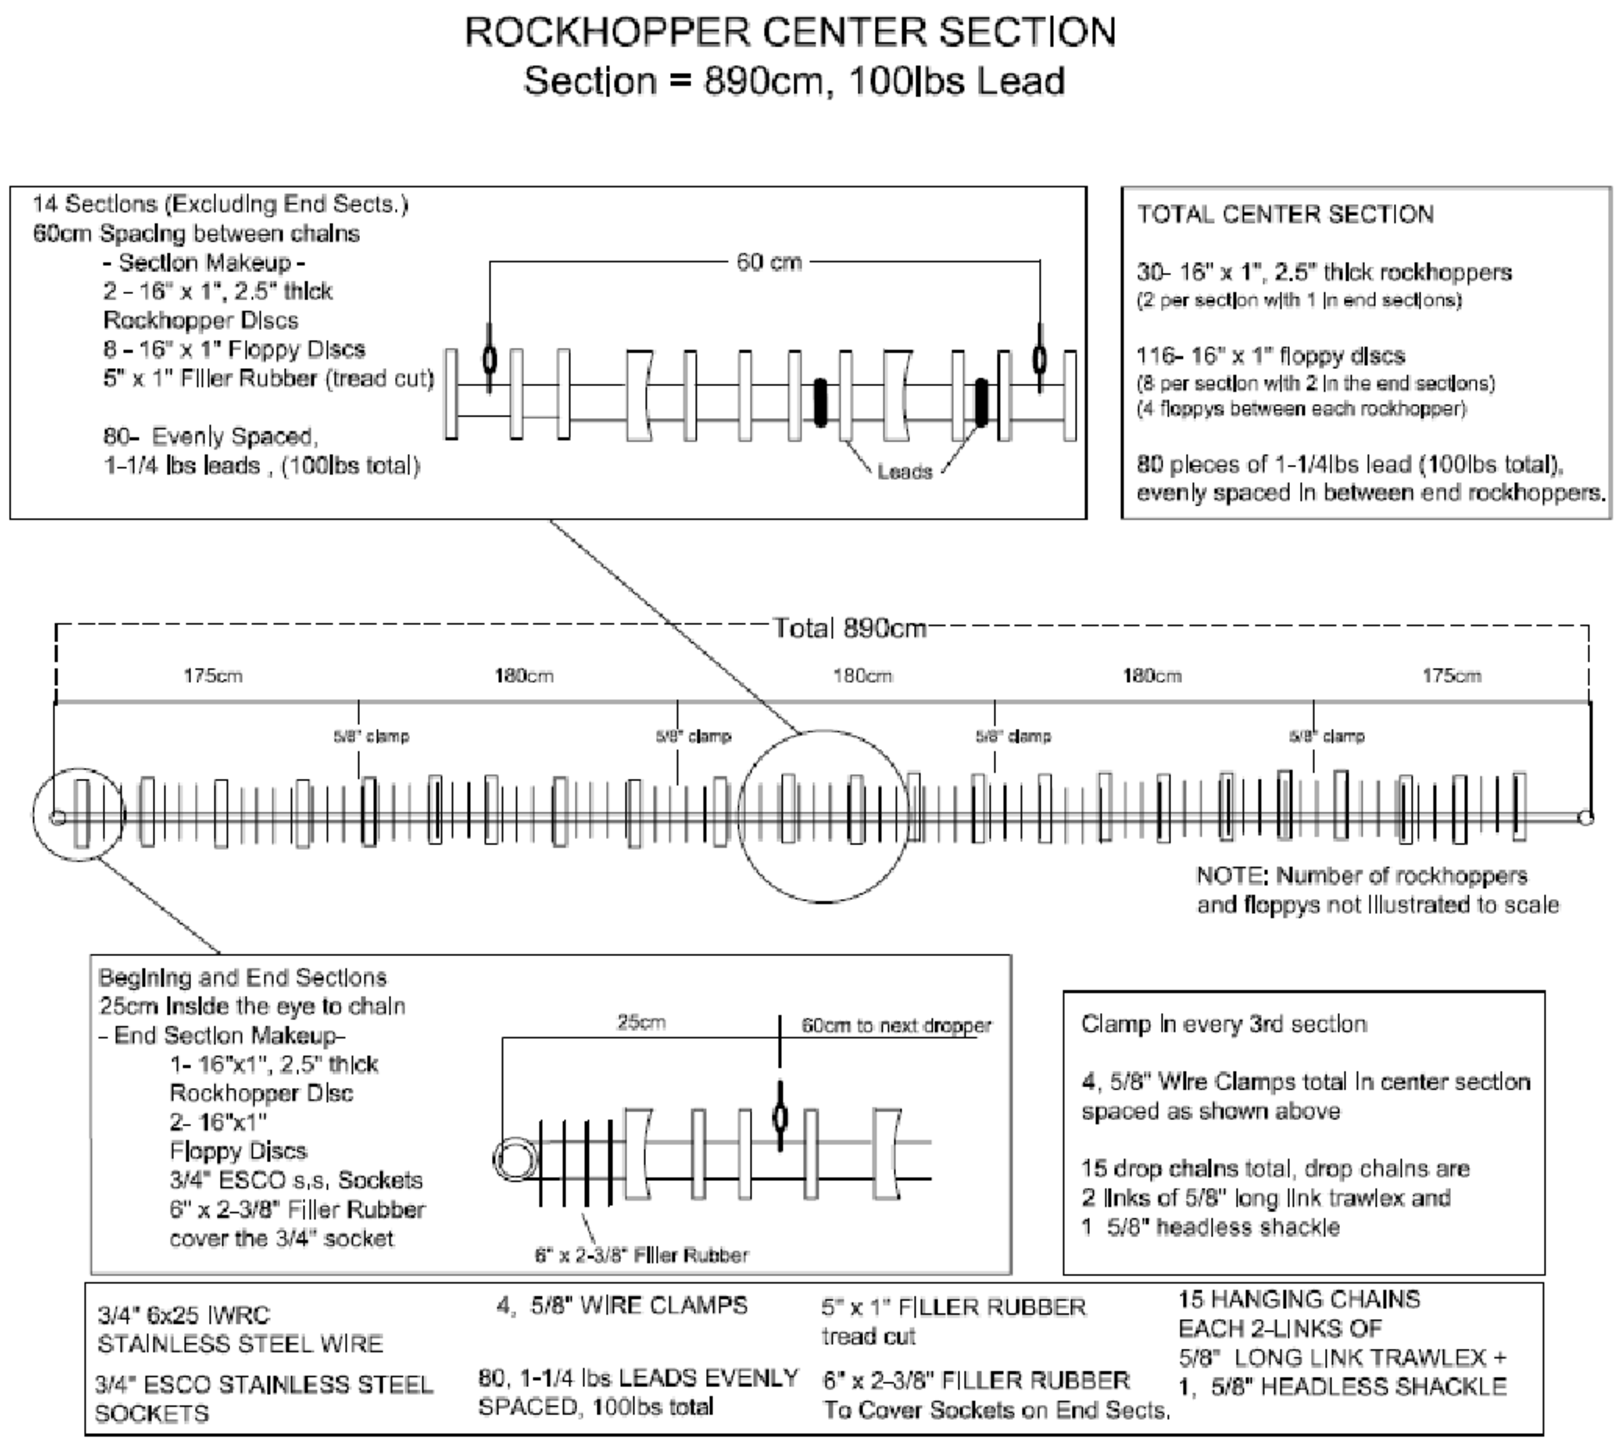
\includegraphics[width = 0.7\textwidth]{rockhopper_schematic_1.pdf}
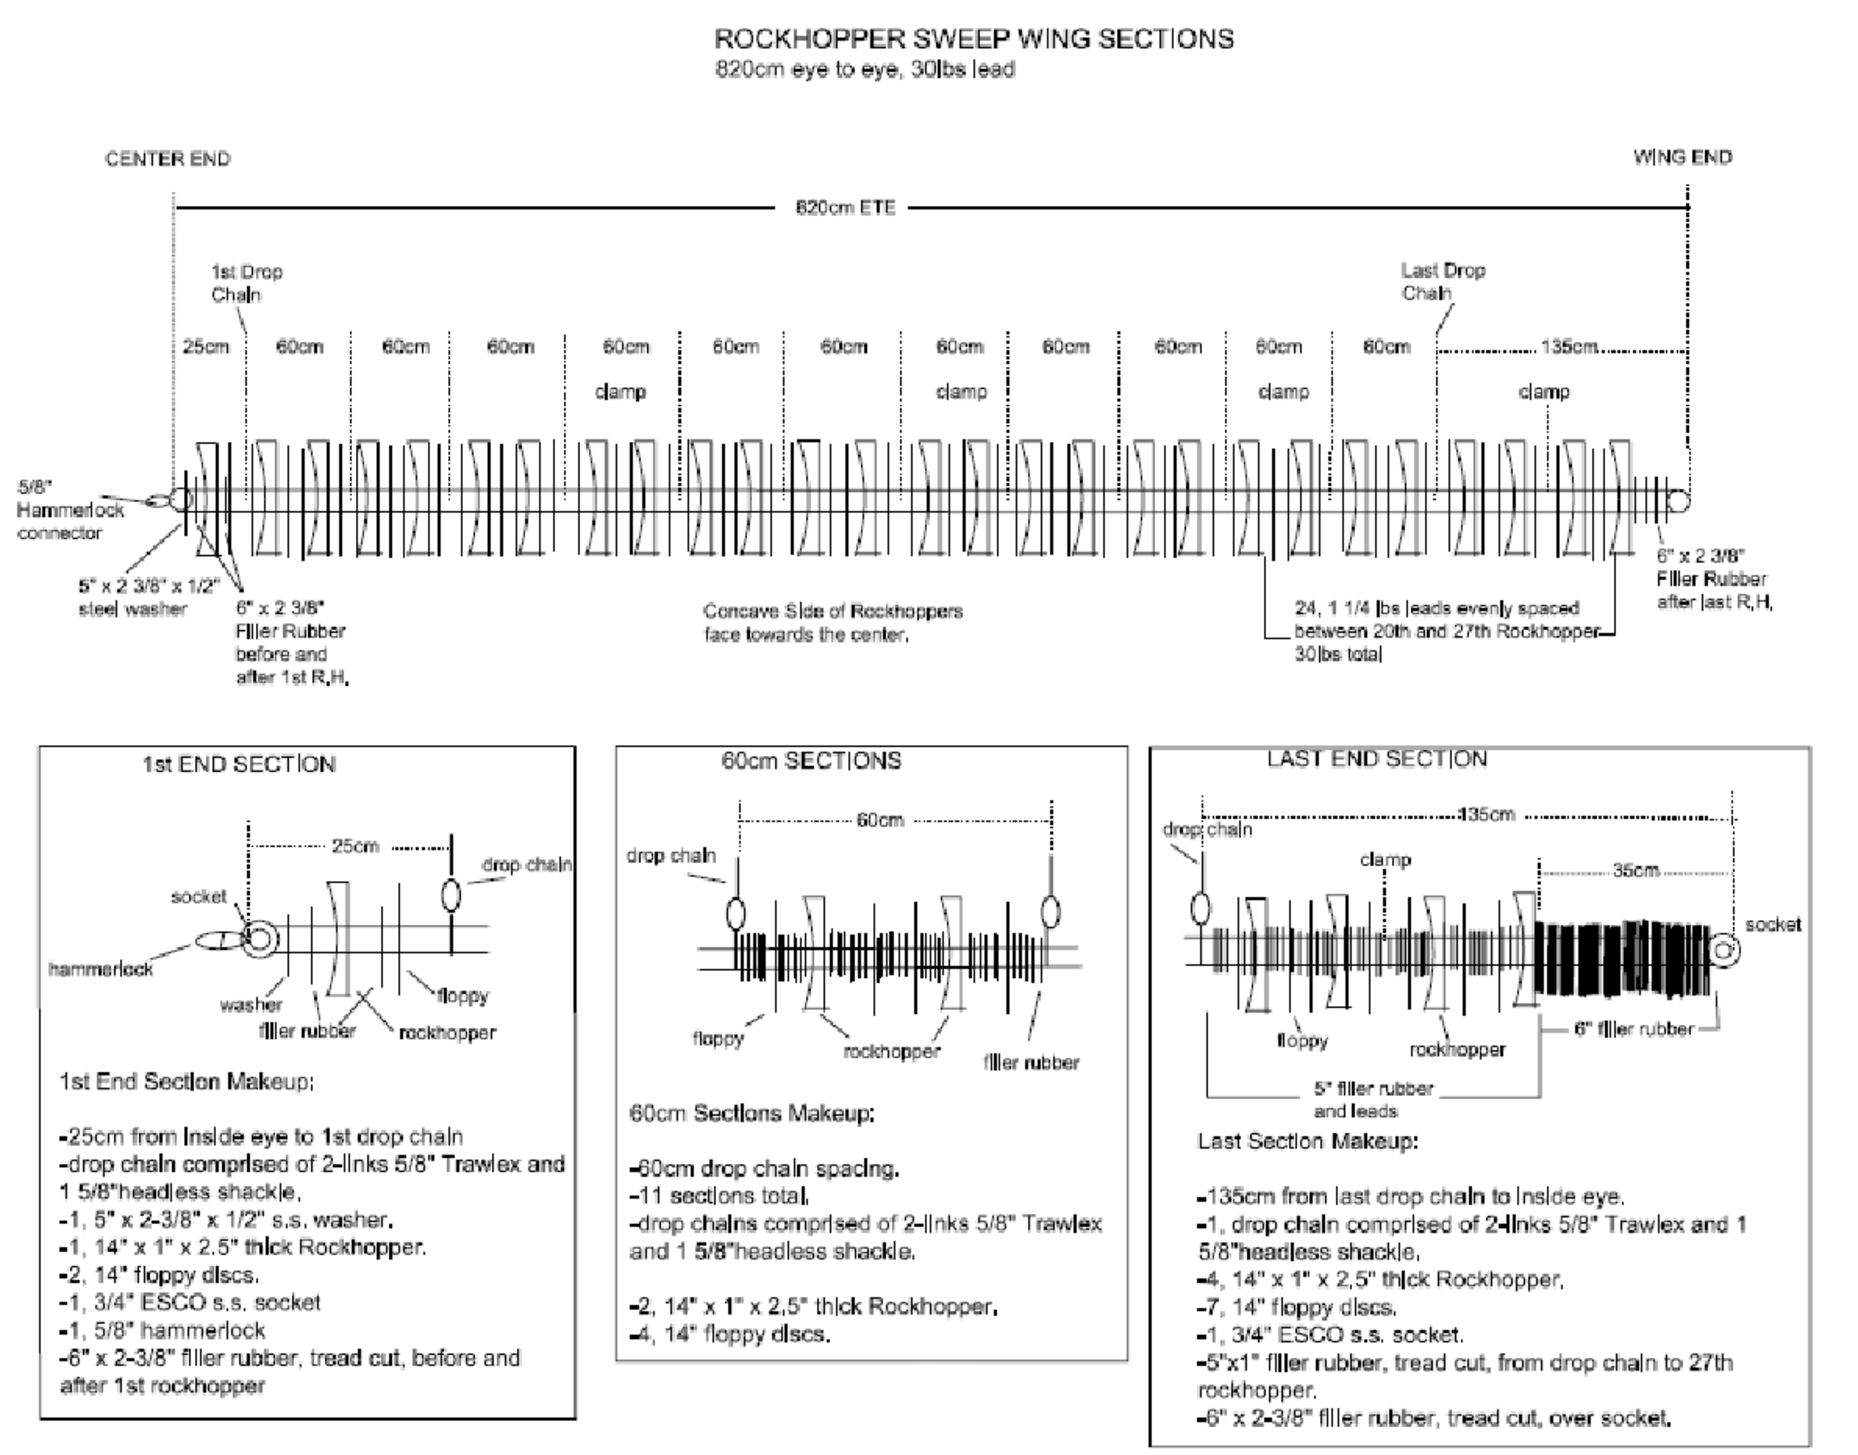
\includegraphics[width = 0.7\textwidth]{rockhopper_schematic_2.pdf}
\end{center}
\end{figure}

\begin{figure}
\caption{Diagram of the chain sweep designed maximize bottom contact and flatfish capture.}\label{chainsweep_schematic}
\begin{center}
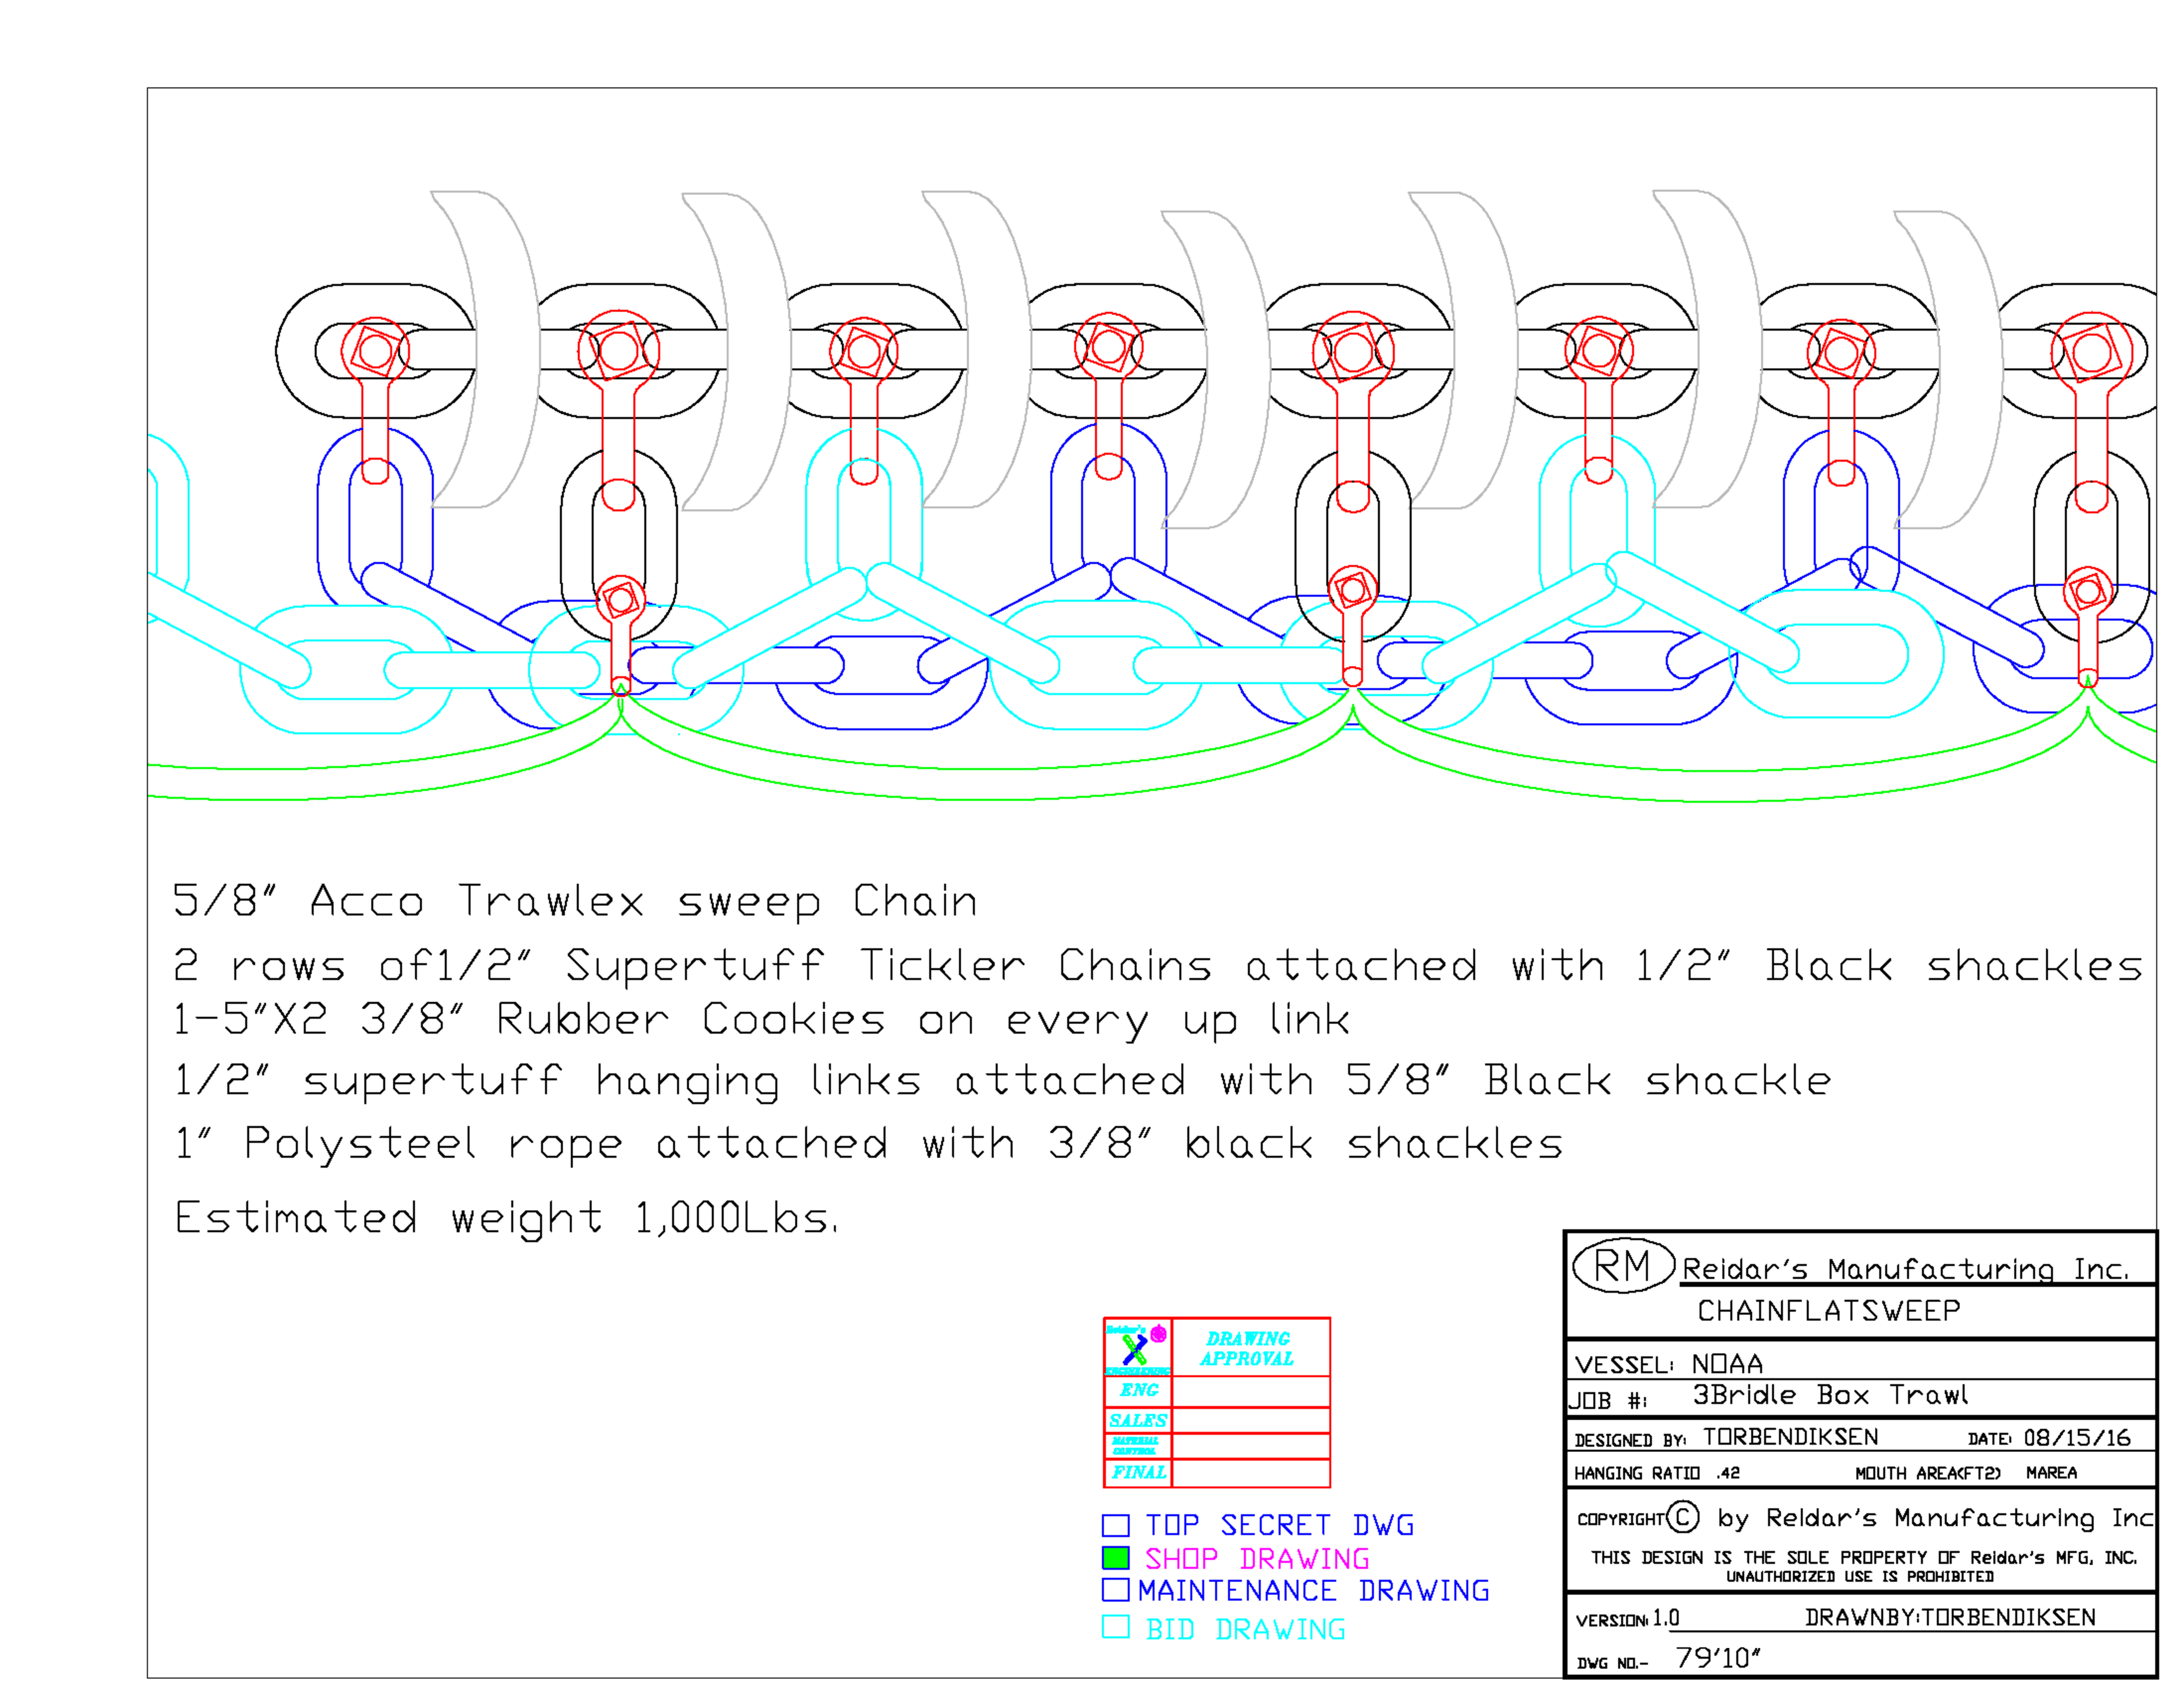
\includegraphics[width = \textwidth]{chainsweep_schematic.pdf}
\end{center}
\end{figure}
\clearpage

\begin{figure}
\caption{Locations of stations in 2015 where the F/V Karen Elizabeth conducted twin-trawl sets with the standard bottom trawl gear and the gear with a chain sweep instead of the rockhopper sweep.}\label{2015_tow_locations}
\begin{center}
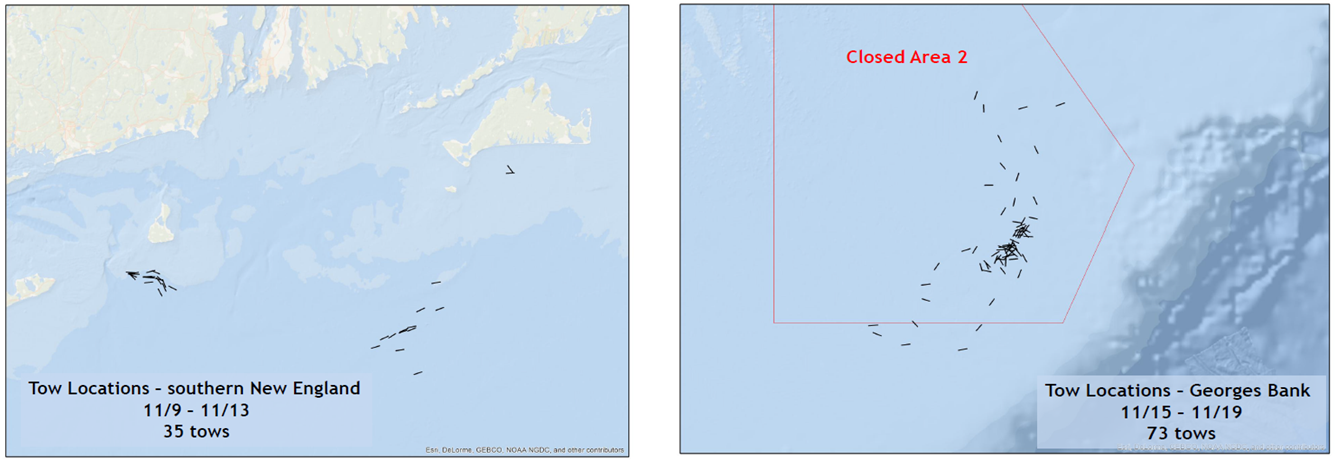
\includegraphics[width = \textwidth]{2015_tow_locations.png}
\end{center}
\end{figure}

\begin{figure}
\caption{Locations of stations in 2016 where the F/V Karen Elizabeth conducted twin-trawl sets with the standard bottom trawl gear and the gear with a chain sweep instead of the rockhopper sweep.}\label{2016_tow_locations}
\begin{center}
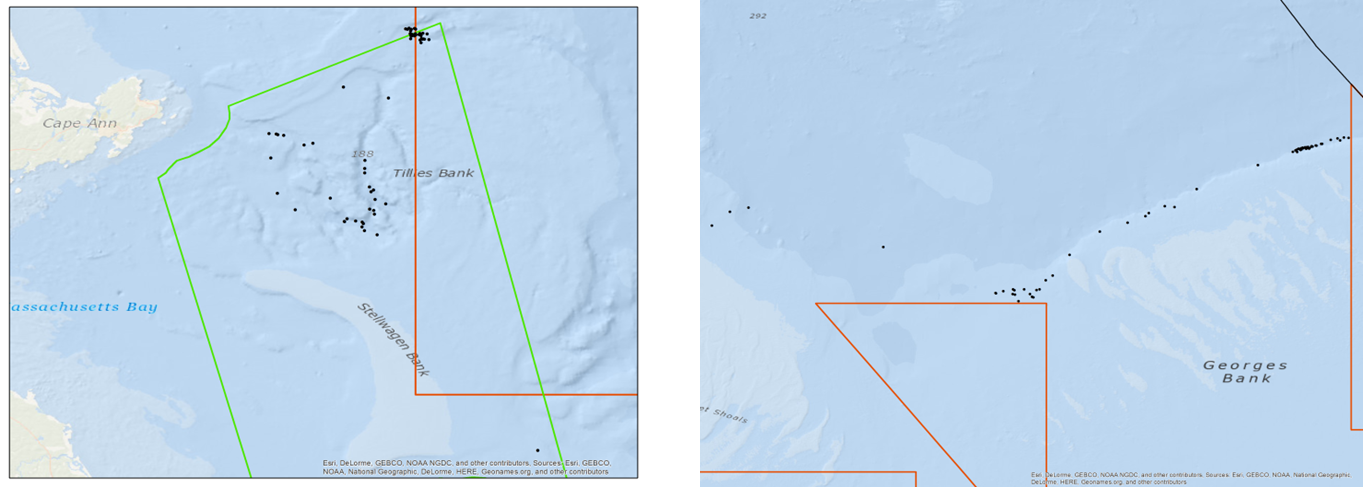
\includegraphics[width = \textwidth]{2016_tow_locations.png}
\end{center}
\end{figure}

\begin{figure}
\caption{Locations of stations in 2017 where the F/V Karen Elizabeth conducted twin-trawl sets with the standard bottom trawl gear and the gear with a chain sweep instead of the rockhopper sweep.}\label{2017_tow_locations}
\begin{center}
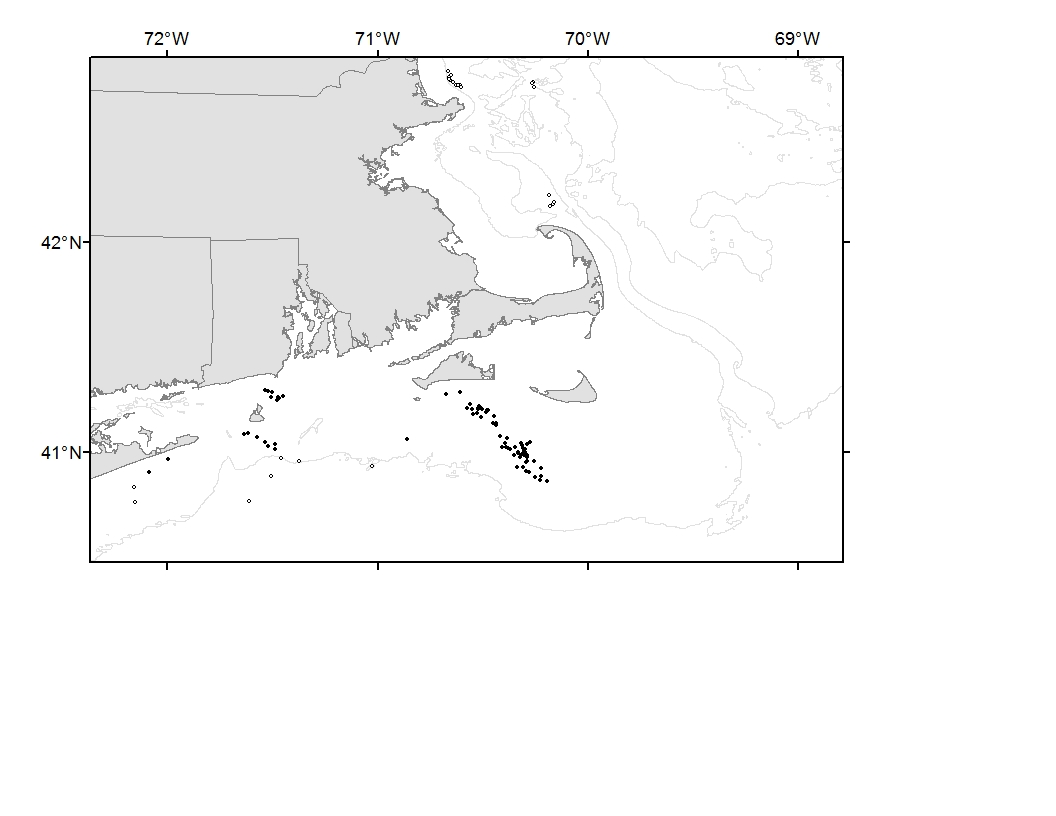
\includegraphics[width = \textwidth]{2017_tow_locations.png}
\end{center}
\end{figure}

\clearpage

\begin{figure}
\caption{Relative efficiency  of gears using chain and rockhopper sweeps from the best performing model for each species (Table \ref{best_model_compare}). Blue and red denote results for day and night data, respectively, and thick and thin lines represent overall and paired-tow specific estimates of relative catch efficiency, respectively. Points represent empirical estimates of relative efficiency for paired observation by length and paired tow. Polygons and dashed lines represent hessian-based and bootstrap-based 95\% confidence intervals, respectively.}\label{sp_rho_plot}
\begin{center}
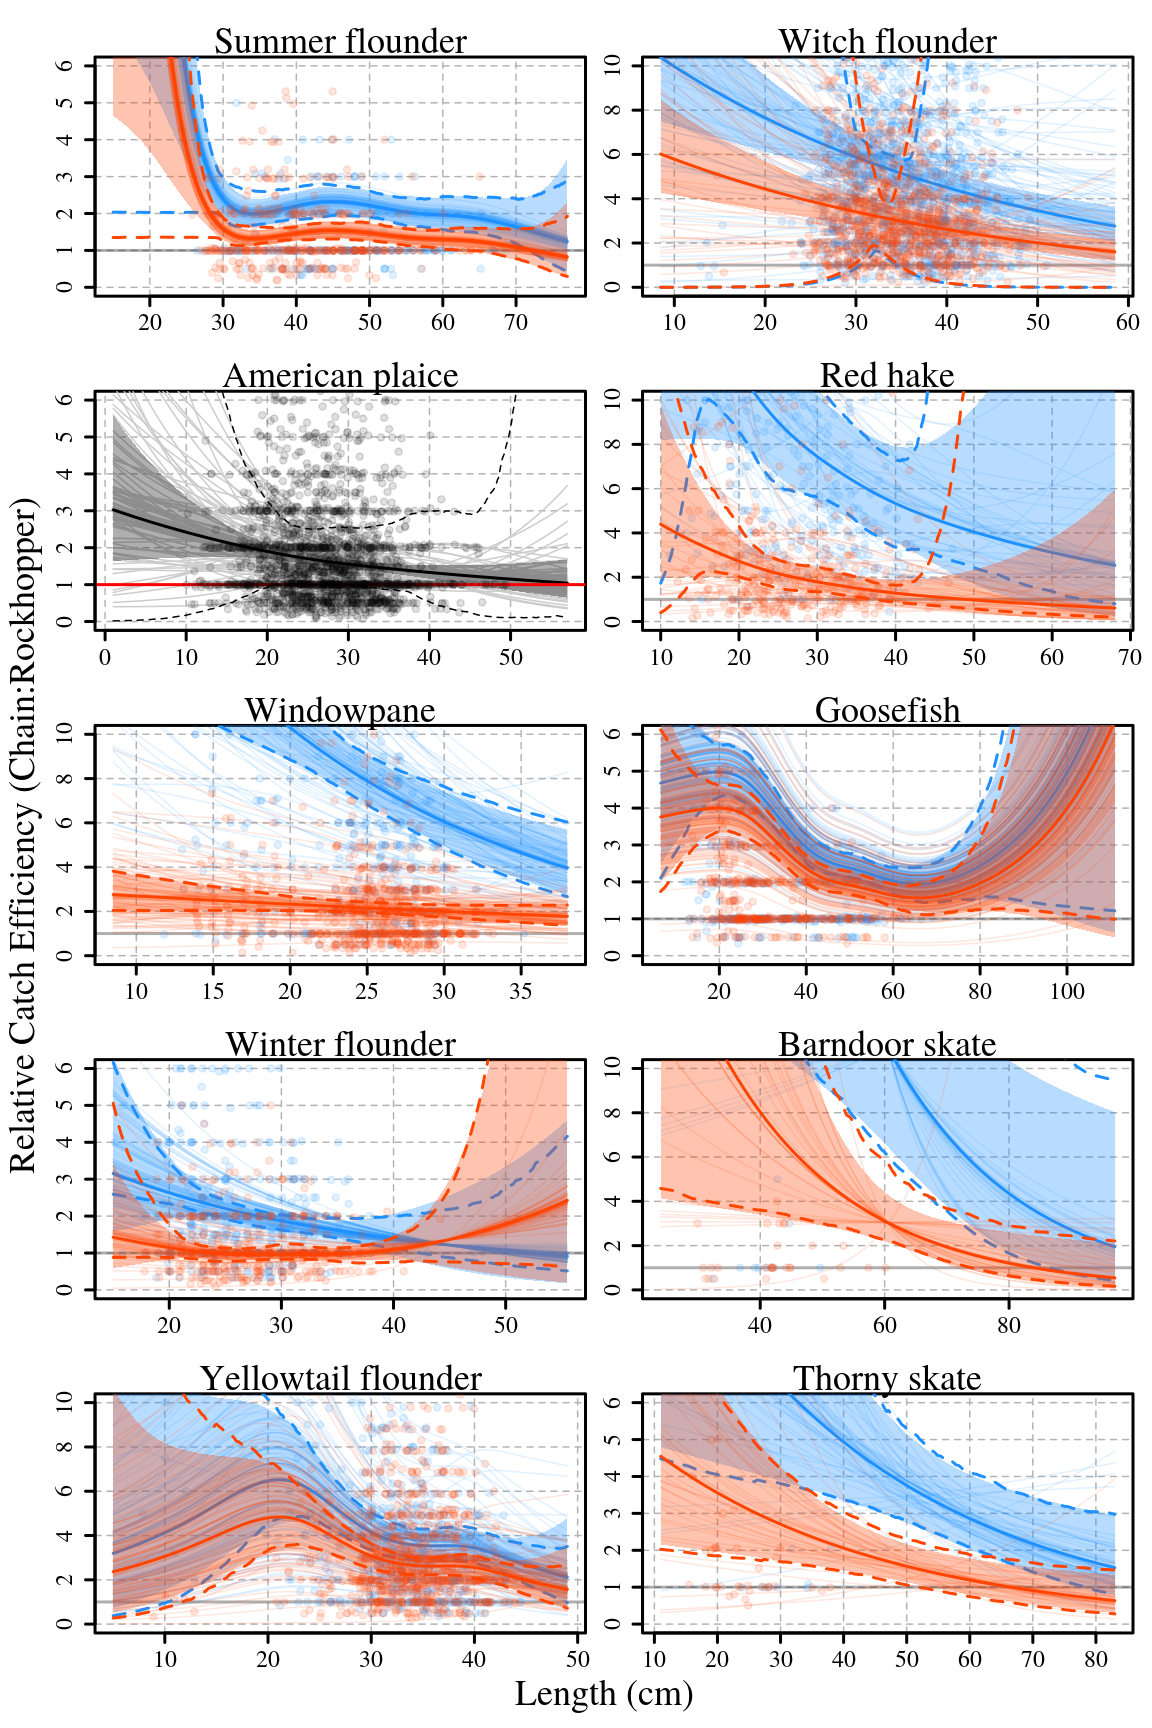
\includegraphics[height = 0.8\textheight]{sp_rho_plot.pdf}
\end{center}
\end{figure}

\clearpage

\begin{figure}
\caption{Annual spring (blue) and fall (red) biomass estimates for each managed stock assuming 100\% efficiency for chainsweep gear with shaded polygons representing bootstrap-based 95\% confidence intervals. Relative catch efficiency at size estimates and bootstraps are from the best performing model for each species (Table \ref{best_model_compare}).}\label{stock_biomass_plot}
\begin{center}
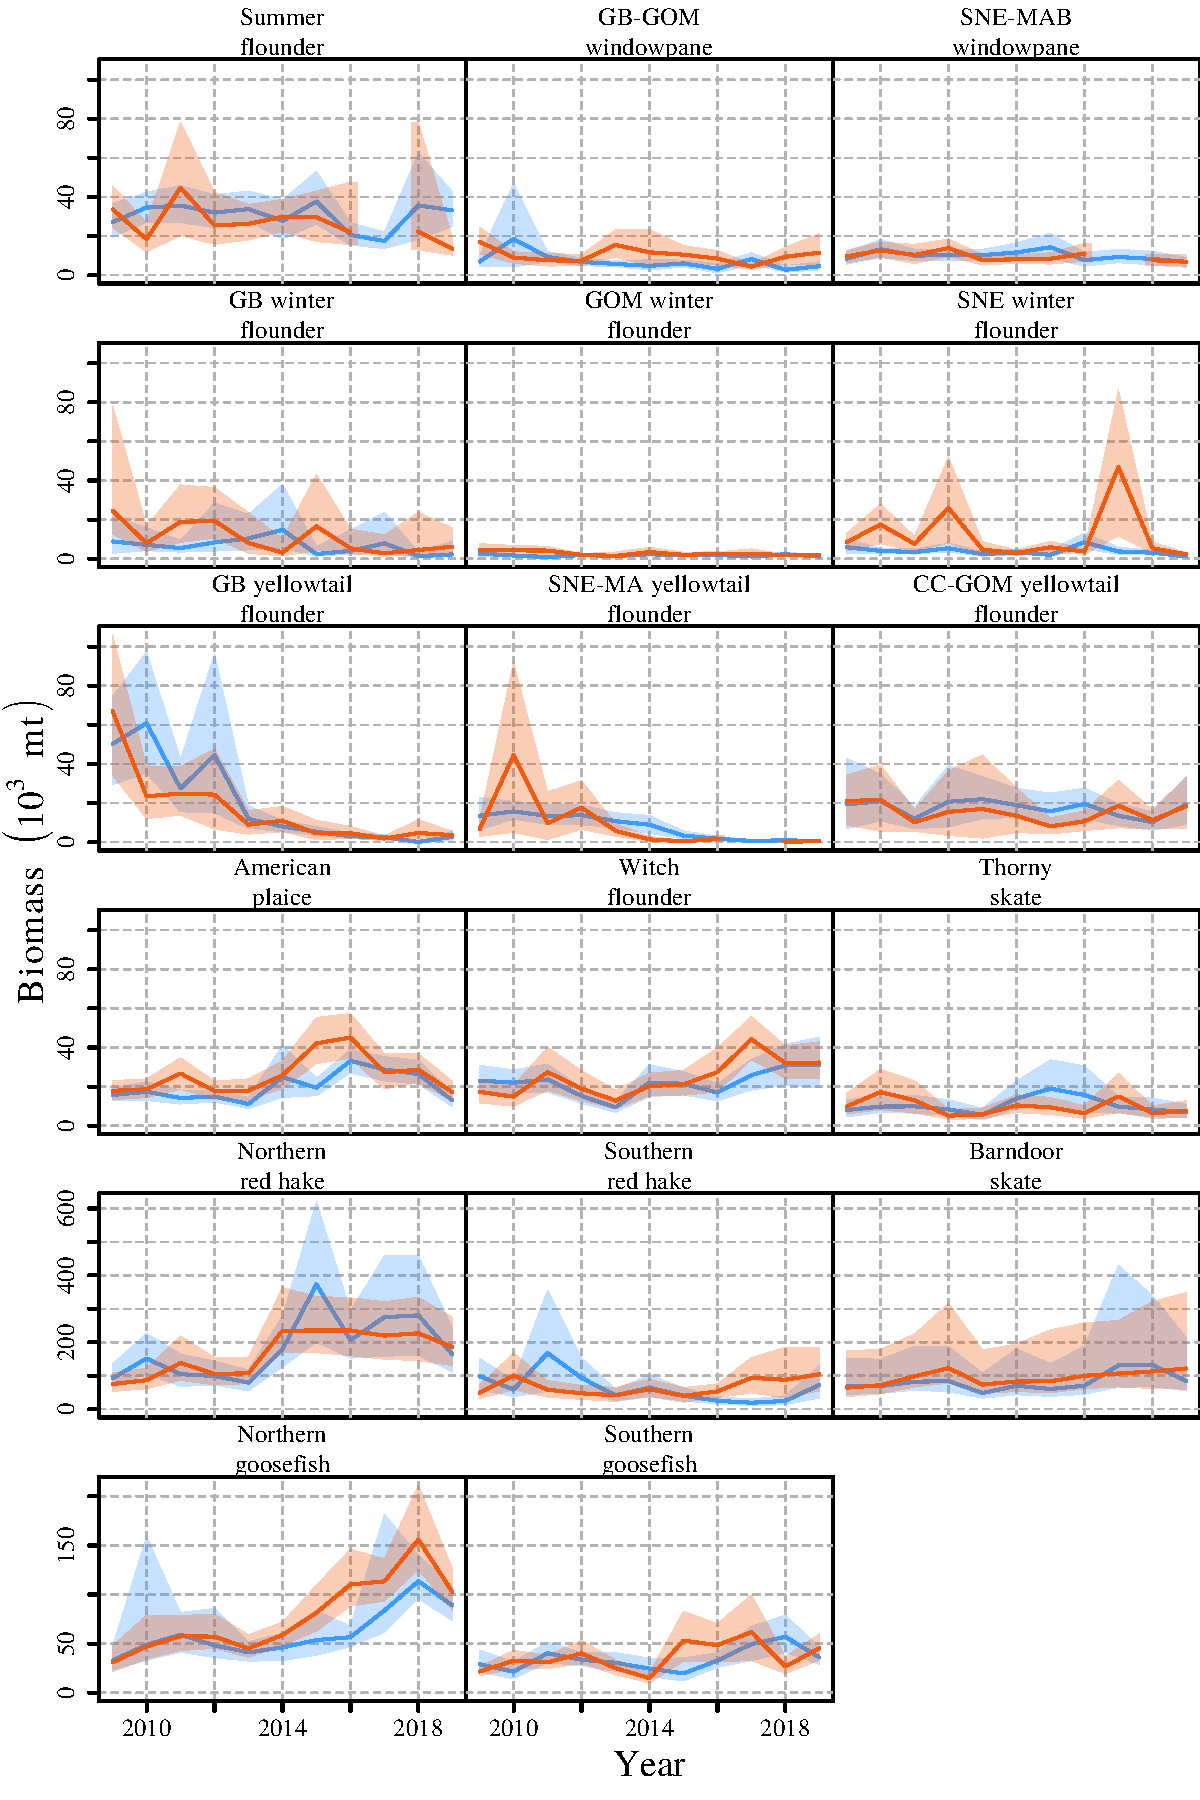
\includegraphics[height = 0.8\textheight]{stock_biomass_plot.pdf}
\end{center}
\end{figure}

\begin{table}
\caption{Managed stocks associated with the species for which relative catch efficiency was estimated.}\label{stock_definition_table}
{%latex.default(stock.definition.table, file = paste0("paper/stock_definition_table.tex"),     first.hline.double = FALSE, col.just = rep("l", 2), table.env = FALSE)%
\begin{center}
\begin{tabular}{l}
\hline
\multicolumn{1}{c}{Stock}\tabularnewline
\hline
Summer flounder\tabularnewline
American Plaice\tabularnewline
Georges Bank-Gulf of Maine (GB-GOM) windowpane\tabularnewline
Southern New England-Mid-Atlantic Bight (SNE-MAB) windowpane\tabularnewline
Georges Bank (GB) winter flounder\tabularnewline
Gulf of Maine (GOM) winter flounder\tabularnewline
Southern New England (SNE) winter flounder\tabularnewline
GB yellowtail flounder\tabularnewline
Southern New England-Mid-Atlantic (SNE-MA) yellowtail flounder\tabularnewline
Cape Cod-Gulf of Maine (CC-GOM) yellowtail flounder\tabularnewline
Witch flounder\tabularnewline
Northern red hake\tabularnewline
Southern red hake\tabularnewline
Northern goosefish\tabularnewline
Southern goosefish\tabularnewline
Barndoor skate\tabularnewline
Thorny skate\tabularnewline
\hline
\end{tabular}\end{center}
}
\end{table}

\begin{landscape}
\begin{table}
\caption{Description of relative catch efficiency ($\rho$) and beta-binomial dispersion ($\phi$) parameterizations for binomial and beta-binomial models and number of marginal likelihood parameters ($n_p$) for the 13 base models from \citet{miller13} and fit to paired chainsweep and rockhoppersweep tow data for each species.}\label{base_model_description}
{%latex.default(out, file = paste0(parentdir, "/paper/base_model_description.tex"),     table.env = FALSE, col.just = c("l", "l", "l", "r", "p{0.5\\textwidth}"),     rowname = NULL)%
\begin{center}
\begin{tabular}{lllrp{0.5\textwidth}}
\hline\hline
\multicolumn{1}{c}{Model}&\multicolumn{1}{c}{$\log\left(\rho\right)$}&\multicolumn{1}{c}{$\log\left(\phi\right)$}&\multicolumn{1}{c}{$n_p$}&\multicolumn{1}{c}{Description}\tabularnewline
\hline
BI$_{0}$&$\sim$ 1&--&$ 1$&population-level mean for all observations\tabularnewline
BI$_{1}$&$\sim$ 1 + 1$|$pair&--&$ 2$&population- and random station-level $\rho$\tabularnewline
BI$_{2}$&$\sim$ s(length)&--&$ 3$&population-level smooth size effect on $\rho$\tabularnewline
BI$_{3}$&$\sim$ s(length) + 1$|$pair&--&$ 4$&population-level smooth size effect and random station-level intercept for $\rho$\tabularnewline
BI$_{4}$&$\sim$ s(length) + s(length)$|$pair&--&$ 7$&population-level and random station-level smooth size effects for $\rho$\tabularnewline
BB$_{0}$&$\sim$ 1&$\sim$ 1&$ 2$&population-level $\rho$ and $\phi$\tabularnewline
BB$_{1}$&$\sim$ 1 + 1$|$pair&$\sim$ 1&$ 3$&population-level and random station-level intercept for $\rho$ and population-level $\phi$\tabularnewline
BB$_{2}$&$\sim$ s(length)&$\sim$ 1&$ 4$&population-level smooth size effect on $\rho$ and population-level $\phi$\tabularnewline
BB$_{3}$&$\sim$ s(length)&$\sim$ s(length)&$ 6$&population-level smooth size effect on $\rho$ and $\phi$\tabularnewline
BB$_{4}$&$\sim$ s(length) + 1$|$pair&$\sim$ 1&$ 5$&population-level smooth size effect and random station-level intercept for $\rho$ and population-level $\phi$\tabularnewline
BB$_{5}$&$\sim$ s(length) + 1$|$pair&$\sim$ s(length)&$ 7$&population-level smooth size effect on $\rho$ and $\phi$ and random station-level intercepts for $\rho$\tabularnewline
BB$_{6}$&$\sim$ s(length) + s(length)$|$pair&$\sim$ 1&$ 8$&population-level and random station-level smooth size effects on $\rho$ and population-level $\phi$\tabularnewline
BB$_{7}$&$\sim$ s(length) + s(length)$|$pair&$\sim$ s(length)&$10$&population-level and random station-level smooth size effects on $\rho$ and population-level smooth size effects on $\phi$\tabularnewline
\hline
\end{tabular}\end{center}
}
\end{table}
\end{landscape}

\begin{landscape}
\begin{table}
\caption{Number of paired tows where fish were captured and the number of fish captured and measured for lengths for each species in total and by day or night.}\label{data_table}
{\fontsize{10pt}{10pt}\selectfont%latex.default(nobs.table, file = paste0(parentdir, "/paper/data_table.tex"),     cgroup = c("Paired Tows", "Captured", "\\thead{Both Gears \\\\ Measured}",         "\\thead{Chainsweep \\\\ Measured}", "\\thead{Rockhopper \\\\ Measured}"),     first.hline.double = FALSE, n.cgroup = c(3, 1, 3, 3, 3),     col.just = rep("r", NCOL(nobs.table)), cgroupTexCmd = "normalfont",     rowlabel = "Species", table.env = FALSE)%
\begin{center}
\begin{tabular}{lrrrcrcrrrcrrrcrrr}
\hline
\multicolumn{1}{l}{\normalfont Species}&\multicolumn{3}{c}{\normalfont Paired Tows}&\multicolumn{1}{c}{\normalfont }&\multicolumn{1}{c}{\normalfont Captured}&\multicolumn{1}{c}{\normalfont }&\multicolumn{3}{c}{\normalfont \thead{Both Gears \\ Measured}}&\multicolumn{1}{c}{\normalfont }&\multicolumn{3}{c}{\normalfont \thead{Chainsweep \\ Measured}}&\multicolumn{1}{c}{\normalfont }&\multicolumn{3}{c}{\normalfont \thead{Rockhopper \\ Measured}}\tabularnewline
\cline{2-4} \cline{6-6} \cline{8-10} \cline{12-14} \cline{16-18}
\multicolumn{1}{l}{}&\multicolumn{1}{c}{Total}&\multicolumn{1}{c}{Day}&\multicolumn{1}{c}{Night}&\multicolumn{1}{c}{}&\multicolumn{1}{c}{Total}&\multicolumn{1}{c}{}&\multicolumn{1}{c}{Total}&\multicolumn{1}{c}{Day}&\multicolumn{1}{c}{Night}&\multicolumn{1}{c}{}&\multicolumn{1}{c}{Total}&\multicolumn{1}{c}{Day}&\multicolumn{1}{c}{Night}&\multicolumn{1}{c}{}&\multicolumn{1}{c}{Total}&\multicolumn{1}{c}{Day}&\multicolumn{1}{c}{Night}\tabularnewline
\hline
Summer flounder&141& 75& 66&& 4,154&& 4,154& 1,770& 2,384&& 2,616&1,195&1,421&&1,538&  575&  963\tabularnewline
American plaice&134& 84& 50&&31,983&&19,245&13,619& 5,626&&10,982&7,775&3,207&&8,263&5,844&2,419\tabularnewline
Windowpane&195&100& 95&&15,310&&13,014& 6,221& 6,793&& 9,854&5,443&4,411&&3,160&  778&2,382\tabularnewline
Winter flounder&171& 97& 74&& 6,586&& 6,449& 3,605& 2,844&& 3,805&2,385&1,420&&2,644&1,220&1,424\tabularnewline
Yellowtail flounder&192&101& 91&&18,545&&14,134& 6,849& 7,285&&10,065&5,297&4,768&&4,069&1,552&2,517\tabularnewline
Witch flounder&132& 83& 49&&57,133&&23,927&13,899&10,028&&14,899&9,271&5,628&&9,028&4,628&4,400\tabularnewline
Red hake& 73& 40& 33&&47,275&&12,585& 6,614& 5,971&& 8,587&4,908&3,679&&3,998&1,706&2,292\tabularnewline
Goosefish&302&165&137&& 8,798&& 8,541& 3,985& 4,556&& 6,409&3,053&3,356&&2,132&  932&1,200\tabularnewline
Barndoor skate& 62& 33& 29&&   502&&   502&   219&   283&&   397&  198&  199&&  105&   21&   84\tabularnewline
Thorny skate& 90& 56& 34&&   907&&   907&   399&   508&&   648&  311&  337&&  259&   88&  171\tabularnewline
\hline
\end{tabular}\end{center}
}
\end{table}
\end{landscape}

\begin{landscape}
\begin{table}\caption{Difference in AIC for each of the 13 models described in Table \ref{base_model_description} from the best model ($\bf 0$) by species.}\label{base_model_compare}
{%latex.default(x, file = paste0(parentdir, "/paper/base_model_compare.tex"),     col.just = rep("r", NCOL(x)), numeric.dollar = FALSE, cellTexCmds = cell.format,     rowlabel = "", table.env = FALSE)%
\begin{center}
\begin{tabular}{lrrrrrrrrrrrrr}
\hline\hline
\multicolumn{1}{l}{}&\multicolumn{1}{c}{BI$_{0}$}&\multicolumn{1}{c}{BI$_{1}$}&\multicolumn{1}{c}{BI$_{2}$}&\multicolumn{1}{c}{BI$_{3}$}&\multicolumn{1}{c}{BI$_{4}$}&\multicolumn{1}{c}{BB$_{0}$}&\multicolumn{1}{c}{BB$_{1}$}&\multicolumn{1}{c}{BB$_{2}$}&\multicolumn{1}{c}{BB$_{3}$}&\multicolumn{1}{c}{BB$_{4}$}&\multicolumn{1}{c}{BB$_{5}$}&\multicolumn{1}{c}{BB$_{6}$}&\multicolumn{1}{c}{BB$_{7}$}\tabularnewline
\hline
   Summer flounder&   27.96&   13.53&   8.9&\bfseries   0&   &   28.64&   15.45&   10.59&   &   &   &   &   \tabularnewline
   American plaice&   821.11&   546.54&   743.34&   494.92&   415.63&   179.48&   71.76&   141.44&   &   37.06&   &   0.71&\bfseries   0\tabularnewline
   Windowpane&   1045.06&   38.51&   1029.72&   17.03&\bfseries   0&   585.7&   32.22&   572.73&   &   15.27&   &   &   \tabularnewline
   Winter flounder&   216.47&   15.73&   200.33&   3.02&\bfseries   0&   163.31&   16.63&   151.66&   151.01&   4.21&   6.78&   1.41&   \tabularnewline
   Yellowtail flounder&   727.15&   97.93&   727.36&   51.84&   10.96&   394.94&   70.2&   391.13&   371.13&   31.85&   &\bfseries   0&   3.33\tabularnewline
   Witch flounder&   1424.17&   212.64&   1372.66&   &   35.33&   881.28&   142.53&   844.47&   &   81.37&   &\bfseries   0&   \tabularnewline
   Red hake&   1884.51&   295.85&   1697.48&   170.75&   &   627.33&   166.43&   590.92&   &   95.8&   59.31&\bfseries   0&   0.83\tabularnewline
   Goosefish&   227.67&   87.23&   80.37&\bfseries   0&   &   219.13&   &   76.54&   &   &   &   &   \tabularnewline
   Barndoor skate&   36.51&   10.01&   31.34&   2.72&\bfseries   0&   36.23&   11.99&   29.03&   &   4.6&   &   &   \tabularnewline
   Thorny skate&   39.04&   8.57&   32.65&   3.44&   1.15&   22.38&   5.84&   18.66&   &   1.38&   5.19&\bfseries   0&   \tabularnewline
\hline
\end{tabular}\end{center}
}
\end{table}
\end{landscape}

\begin{landscape}
\begin{table}\caption{Best performing models from Table \ref{base_model_compare} and extended models that include diel effects on relative catch efficiency for each species with the number of parameters for each model ($n_p$) and the differences in AIC ($\Delta$AIC) from the best of the three models ($\bf 0$) by species.}\label{best_model_compare}
{\fontsize{7pt}{7pt}\selectfont%latex.default(temp, file = paste0(parentdir, "/paper/best_model_compare.tex"),     rgroup = sp.info$sp.pretty.names[ind], n.rgroup = rep(3,         length(ind)), col.just = c("l", "l", "l", rep("r", 2)),     numeric.dollar = FALSE, cellTexCmds = cell.format, rowlabel = "",     rowname = rep("", NROW(temp)), table.env = FALSE)%
\begin{center}
\begin{tabular}{llllrr}
\hline\hline
\multicolumn{1}{l}{}&\multicolumn{1}{c}{Model}&\multicolumn{1}{c}{$\log\left(\rho\right)$}&\multicolumn{1}{c}{$\log\left(\phi\right)$}&\multicolumn{1}{c}{$n_p$}&\multicolumn{1}{c}{$\Delta$AIC}\tabularnewline
\hline
{\bfseries Summer flounder}&&&&&\tabularnewline
   ~~&   BI$_{3}$&   $\sim$ s(length) + 1$|$pair&   --&    4&   22.92\tabularnewline
   ~~&   BI$_{3a}$&   $\sim$ dn + s(length) + 1$|$pair&   --&    5&\bfseries   0\tabularnewline
   ~~&   BI$_{3b}$&   $\sim$ dn * s(length) + 1$|$pair&   --&    7&   1.74\tabularnewline
\hline
{\bfseries American plaice}&&&&&\tabularnewline
   ~~&   BB$_{7}$&   $\sim$ s(length) + s(length)$|$pair&   $\sim$ s(length)&   10&\bfseries   0\tabularnewline
   ~~&   BB$_{7a}$&   $\sim$ dn + s(length) + s(length)$|$pair&   $\sim$ s(length)&   11&   1.43\tabularnewline
   ~~&   BB$_{7b}$&   $\sim$ dn * s(length) + s(length)$|$pair&   $\sim$ s(length)&   13&   2.95\tabularnewline
\hline
{\bfseries Windowpane}&&&&&\tabularnewline
   ~~&   BI$_{4}$&   $\sim$ s(length) + s(length)$|$pair&   --&    7&   152.1\tabularnewline
   ~~&   BI$_{4a}$&   $\sim$ dn + length + s(length)$|$pair&   --&    7&   4.06\tabularnewline
   ~~&   BI$_{4b}$&   $\sim$ dn * length + s(length)$|$pair&   --&    8&\bfseries   0\tabularnewline
\hline
{\bfseries Winter flounder}&&&&&\tabularnewline
   ~~&   BI$_{4}$&   $\sim$ s(length) + s(length)$|$pair&   --&    7&   50.68\tabularnewline
   ~~&   BI$_{4a}$&   $\sim$ dn + s(length) + length$|$pair&   --&    7&   0.3\tabularnewline
   ~~&   BI$_{4b}$&   $\sim$ dn * s(length) + length$|$pair&   --&    9&\bfseries   0\tabularnewline
\hline
{\bfseries Yellowtail flounder}&&&&&\tabularnewline
   ~~&   BB$_{6}$&   $\sim$ s(length) + s(length)$|$pair&   $\sim$ 1&    8&   3.84\tabularnewline
   ~~&   BB$_{6a}$&   $\sim$ dn + s(length) + s(length)$|$pair&   $\sim$ 1&    9&\bfseries   0\tabularnewline
   ~~&   BB$_{6b}$&   $\sim$ dn * s(length) + s(length)$|$pair&   $\sim$ 1&   11&   3.48\tabularnewline
\hline
{\bfseries Witch flounder}&&&&&\tabularnewline
   ~~&   BB$_{6}$&   $\sim$ s(length) + s(length)$|$pair&   $\sim$ 1&    8&   19.68\tabularnewline
   ~~&   BB$_{6a}$&   $\sim$ dn + length + s(length)$|$pair&   $\sim$ 1&    8&\bfseries   0\tabularnewline
   ~~&   BB$_{6b}$&   $\sim$ dn * length + s(length)$|$pair&   $\sim$ 1&    9&   1.52\tabularnewline
\hline
{\bfseries Red hake}&&&&&\tabularnewline
   ~~&   BB$_{6}$&   $\sim$ s(length) + s(length)$|$pair&   $\sim$ 1&    8&   32.35\tabularnewline
   ~~&   BB$_{6a}$&   $\sim$ dn + s(length) + s(length)$|$pair&   $\sim$ 1&    8&\bfseries   0\tabularnewline
   ~~&   BB$_{6b}$&   $\sim$ dn * s(length) + s(length)$|$pair&   $\sim$ 1&   10&   3.18\tabularnewline
\hline
{\bfseries Goosefish}&&&&&\tabularnewline
   ~~&   BI$_{3}$&   $\sim$ s(length) + 1$|$pair&   --&    4&   5.44\tabularnewline
   ~~&   BI$_{3a}$&   $\sim$ dn + s(length) + 1$|$pair&   --&    5&\bfseries   0\tabularnewline
   ~~&   BI$_{3b}$&   $\sim$ dn * s(length) + 1$|$pair&   --&    7&   6.8\tabularnewline
\hline
{\bfseries Barndoor skate}&&&&&\tabularnewline
   ~~&   BI$_{4}$&   $\sim$ s(length) + s(length)$|$pair&   --&    7&   15.57\tabularnewline
   ~~&   BI$_{4a}$&   $\sim$ dn + length + length$|$pair&   --&    5&\bfseries   0\tabularnewline
   ~~&   BI$_{4b}$&   $\sim$ dn * length + length$|$pair&   --&    6&   1.83\tabularnewline
\hline
{\bfseries Thorny skate}&&&&&\tabularnewline
   ~~&   BB$_{6}$&   $\sim$ s(length) + s(length)$|$pair&   $\sim$ 1&    8&   15.51\tabularnewline
   ~~&   BB$_{6a}$&   $\sim$ dn + length + length$|$pair&   $\sim$ 1&    7&\bfseries   0\tabularnewline
   ~~&   BB$_{6b}$&   $\sim$ dn * length + length$|$pair&   $\sim$ 1&    8&   1.38\tabularnewline
\hline
\end{tabular}\end{center}
}
\end{table}
\end{landscape}

\begin{table}
\caption{Average of annual (2009-2019) ratios of coefficients of variation for calibrated and uncalibrated biomass indices for each stock by seasonal survey. Coefficients of variation are based on bootstrap resampling of paired tow observations, survey station data and associated length and weight observations. Annual indices for fall 2017 were not available for summer flounder, SNE-MA windowpane, and SNE-MA yellowtail flounder.}\label{stock_cv_ratios}
{%latex.default(round(cv.ratios[stock.order, 2:1], 2), file = paste0(parentdir,     "/paper/stock_cv_ratios.tex"), cgroup = c("\\thead{Average CV Ratio \\\\ Calibrated:Uncalibrated}"),     first.hline.double = FALSE, n.cgroup = 2, collabel.just = rep("r",         2), col.just = rep("r", 2), cgroupTexCmd = "normalfont",     rowlabel = "Stock", table.env = FALSE)%
\begin{center}
\begin{tabular}{lrr}
\hline
\multicolumn{1}{l}{\normalfont Stock}&\multicolumn{2}{c}{\normalfont \thead{Average CV Ratio \\ Calibrated:Uncalibrated}}\tabularnewline
\cline{2-3}
\multicolumn{1}{l}{}&\multicolumn{1}{r}{Spring}&\multicolumn{1}{r}{Fall}\tabularnewline
\hline
Summer flounder&$1.13$&$1.51$\tabularnewline
American plaice&$1.07$&$1.02$\tabularnewline
GB-GOM windowpane&$1.03$&$1.07$\tabularnewline
SNE-MAB windowpane&$1.06$&$0.90$\tabularnewline
GB winter flounder&$3.19$&$3.89$\tabularnewline
GOM winter flounder&$1.05$&$1.07$\tabularnewline
SNE winter flounder&$1.77$&$0.99$\tabularnewline
GB yellowtail flounder&$1.06$&$0.98$\tabularnewline
SNE-MA yellowtail flounder&$1.05$&$0.99$\tabularnewline
CC-GOM yellowtail flounder&$1.01$&$1.02$\tabularnewline
Witch flounder&$1.12$&$1.11$\tabularnewline
Northern red hake&$1.95$&$2.78$\tabularnewline
Southern red hake&$1.28$&$1.28$\tabularnewline
Northern goosefish&$1.93$&$1.34$\tabularnewline
Southern goosefish&$1.18$&$1.04$\tabularnewline
Barndoor skate&$2.47$&$2.78$\tabularnewline
Thorny skate&$1.14$&$1.20$\tabularnewline
\hline
\end{tabular}\end{center}
}
\end{table}

\begin{table}
\caption{Average correlation of annual (2009-2019) calibrated biomass indices for each stock by seasonal survey. Annual indices for fall 2017 were not available for SNE-MA windowpane and SNE-MA yellowtail flounder.}\label{stock_mean_cor}
{%latex.default(round(mean.cor[stock.order, c(3, 1)], 2), file = paste0(parentdir,     "/paper/stock_mean_cor.tex"), first.hline.double = FALSE,     n.cgroup = 2, colheads = c("Spring", "Fall"), rowlabel = "Stock",     table.env = FALSE)%
\begin{center}
\begin{tabular}{lrr}
\hline
\multicolumn{1}{l}{Stock}&\multicolumn{1}{c}{Spring}&\multicolumn{1}{c}{Fall}\tabularnewline
\hline
Summer flounder&$0.16$&$0.14$\tabularnewline
American plaice&$0.09$&$0.06$\tabularnewline
GB-GOM windowpane&$0.06$&$0.04$\tabularnewline
SNE-MAB windowpane&$0.06$&$0.05$\tabularnewline
GB winter flounder&$0.65$&$0.45$\tabularnewline
GOM winter flounder&$0.05$&$0.05$\tabularnewline
SNE winter flounder&$0.07$&$0.03$\tabularnewline
GB yellowtail flounder&$0.05$&$0.04$\tabularnewline
SNE-MA yellowtail flounder&$0.07$&$0.02$\tabularnewline
CC-GOM yellowtail flounder&$0.05$&$0.04$\tabularnewline
Witch flounder&$0.10$&$0.10$\tabularnewline
Northern red hake&$0.42$&$0.34$\tabularnewline
Southern red hake&$0.25$&$0.21$\tabularnewline
Northern goosefish&$0.21$&$0.30$\tabularnewline
Southern goosefish&$0.10$&$0.07$\tabularnewline
Barndoor skate&$0.74$&$0.81$\tabularnewline
Thorny skate&$0.29$&$0.25$\tabularnewline
\hline
\end{tabular}\end{center}
}
\end{table}

\end{document}
